\documentclass[12pt]{article}

\usepackage{ amsmath, amssymb, graphicx, psfrag, bm, multirow }
\usepackage{amsmath,amsthm,amssymb}
\usepackage{mathtools}
\usepackage{tikz}
\usepackage{fancybox}
\usepackage{hyperref}
\usepackage{varwidth}
\usepackage{mdframed}
\usepackage{mathrsfs}
\usepackage[most]{tcolorbox}
\usepackage{accents}
\usepackage{listings}
\graphicspath{ {./images/} }

\addtolength{\textheight}{2.2in}
\addtolength{\topmargin}{-1.3in}
\addtolength{\textwidth}{1.865in}
\addtolength{\oddsidemargin}{-0.95in}
\addtolength{\evensidemargin}{-0.95in}
\setlength{\parskip}{0.15in}
\setlength{\parindent}{0.0in}

\pagestyle{plain}

\raggedbottom

\newcommand{\given}{\, | \,}
\newcommand{\lrp}[1]{\left(#1\right)}
\newcommand{\lrb}[1]{\left[#1\right]}
\newcommand{\lrc}[1]{\left\{#1\right\}}
\newenvironment{solution}{\begin{tcolorbox}[breakable]\begin{proof}[\textbf{\textit{Solution}}] }{\end{proof}\end{tcolorbox}}
\newcommand{\bi}[1]{\textbf{\textit{#1}}}
\renewcommand\labelitemi{$\blacktriangleright$}
\newcommand{\bb}{\mathcal{B}}
\newcommand{\btheta}{\bm{\theta}}
\newcommand{\by}{\bm{y}}
\newcommand{\tcr}[1]{\textcolor{red}{#1}}
\begin{document}

\begin{flushleft}

Prof.~David Draper \\
University of California, Santa Cruz \\
Department of Statistics \\
Baskin School of Engineering \\
Winter 2022

\end{flushleft}

\Large

\begin{center}

STAT 206 (\textsf{Applied Bayesian Statistics})

\hspace*{-0.1in}\fbox{\textbf{Take-Home Test 2}}

\large

(please watch email and \texttt{Canvas} for the final due date)

\end{center}

\normalsize

\textbf{Name:} Kevin Guillen

Here are the (process) ground rules: this test is open-book and open-notes, and
consists of two problems (true/false and calculation); ; \textbf{each of the 6
true/false questions is worth\footnote{Throughout the test, I've tried to be completely clear about the location of each sub-part of each problem by surrounding the possible points with boxes and putting the text inside the boxes in bold italic font.} \fbox{\textit{10 points}}, \vspace*{0.025in} and the calculation problem is worth \fbox{\textit{310 total points}}, for a total of \fbox{\textit{370 points}}}.

Some advice on style as you write up your solutions: pretend that you're sitting next to the grader, having a conversation about problem $( x )$ part $( y )$. You say, ``The answer is $z$,'' and the grader says, ``Why?'' You then give your explanation, as succinctly as possible to get your idea across. The right answer with no reasoning to support it, or incorrect reasoning, will get \textbf{half credit}, so try to make a serious effort on each part of each problem (this will ensure you at least half credit). In an AMS graduate class I taught in 2012, on a take-home test like this one there were 15 true/false questions, worth a total of 150 points; one student got a score of 92 out of 150 (61\%, a D$-$, in a graduate class where B$-$ is the lowest passing grade) on that part of the test, for repeatedly answering just ``true" or ``false" with no explanation. Don't let that happen to you.  

On each problem, the graders and I mentally start everybody out at $-0$ (i.e., with a perfect score), and then you accumulate negative points for incorrect answers and/or reasoning, or parts of problems left blank.

This test is to be entirely your own efforts; do not collaborate with
anyone or get help from anyone but me or our TA (Jacob Fontana). The intent is that the course lecture notes and readings should be sufficient to provide you with all the guidance you need to solve the problems posed below, but you may use other written materials (e.g., the web, journal articles, and books other than those already mentioned in the readings),
\textbf{provided that you cite your sources thoroughly and accurately}; you
will lose (substantial) credit for, e.g., lifting blocks of text directly
from \texttt{wikipedia} and inserting them into your solutions without full
attribution.

If it's clear that (for example) two people have worked together on a part
of a problem that's worth 20 points, and each answer would have earned 16
points if it had not arisen from a collaboration, then each person will
receive 8 of the 16 points collectively earned (for a total score of 8 out
of 20), and I reserve the right to impose additional penalties at my
discretion. If you solve a problem on your own and then share your solution
with anyone else, you're just as guilty of illegal collaboration as
the person who took your solution from you, and both of you will receive
the same penalty. This sort of thing is necessary on behalf of the many
people who do not cheat, to ensure that their scores are meaningfully
earned. In the AMS graduate class in 2012 mentioned above, five people failed the class because of illegal collaboration; don't let that happen to you.

In class I've demonstrated numerical work in \texttt{R}; you can (of course) make the calculations and plots requested in the problems below in any environment you prefer (e.g., \texttt{Matlab}, ...). To avoid plagiarism, if you end up using any of the code I post on the course web page or generate during office hours, at the beginning of your Appendix (see below) you can say something like the following: \vspace*{-0.1in} 

\begin{quote}

\textit{I used some of Prof.~Draper's \texttt{R} code in this assignment, adapting it as needed.} \vspace*{-0.1in} 

\end{quote}

Those of You who are using \texttt{LaTeX} or some other word-processing environment to prepare Your solutions can stick quote blocks below each question, into which You can type Your answers (I suggest that You use \textbf{bold} or \textit{italic} font to distinguish Your solutions from the questions). If You're submitting Your answers in longhand, which is perfectly acceptable, You can just write them out on separate sheets of paper, making sure that the grader can easily figure out which chunk of text is the solution to which part of which problem.

\textbf{Please collect \{all of the code you used in answering the questions  below\} into an Appendix at the end of your document, so that (if you do something wrong) the grader can more accurately give you part credit.} 

\begin{quote}

\bi{NB} The calculation problems in Section 2 look hard just because they're long, but they're not any harder than usual in this class; because of the extremely compressed nature of this course, I have to do a fair amount of teaching in these problems, just to set up the relevant scientific and statistical questions. 

\end{quote}

\section{True/False}

[ \bi{60 total points:~\fbox{10 points each}} ] \vspace*{0.025in} For each statement below, say whether it's true or false; if true without further assumptions, briefly explain why it's true (and what its implications are for statistical inference); if it's sometimes true, give the extra conditions necessary to make it true; if it's false, briefly explain how to change it so that it's true and/or give an example of why it's false. If the statement consists of two or more sub-statements and two or more of them are false, you need to explicitly address all of the false sub-statements in your answer. \vspace*{-0.1in}

\begin{itemize}

\item[(A)]

Consider the sampling model $( Y_i \given \bm{ \theta } \, { \cal B } ) \stackrel{ \textrm{\footnotesize IID} }{ \sim } p ( y_i \given \bm{ \theta } \, { \cal B } )$ for $i = 1, \dots, n$, where the $y_i$ (the observed values of the $Y_i$) are real numbers, $\bm{ \theta }$ is a parameter vector of length $1 \le k < \infty$ and $\cal B$ summarizes Your background information; a Bayesian analysis with the same sampling model would add a prior distribution layer of the form $( \bm{ \theta } \given \mathcal{ B } ) \sim p ( \bm{ \theta } \given \mathcal{ B } )$ to the hierarchy. The Bernstein-von Mises theorem says that maximum-likelihood (ML) and Bayesian inferential conclusions about $\bm{ \theta }$ will be similar in this setting if (a) $n$ is large and (b) $p ( \bm{ \theta } )$ is a low-information (LI) prior, but the theorem does not provide guidance on how large $n$ needs to be for its conclusion to hold in any specific sampling model. \fbox{\textbf{\textit{10 points}}}

\begin{solution}
    This is \textbf{True}, it follows from what we covered today in lecture 2/23. We see it in practice when we compare the likelihood PDF with the posterior PDF when we have low information priors.
\end{solution}

\item[(B)]

In the basic diagram that illustrates the frequentist inferential paradigm
 --- with the population, sample and repeated-sampling data sets, each containing $N$, $n$, and $M$ elements, respectively (see the document camera notes from 20 Jan 2022), and with the sample drawn from the population in an IID manner --- when the population parameter of main interest is the mean $\theta$ and the estimator is the sample mean $\bar{ Y }$, You will always get a Gaussian long-run distribution for $\bar{ Y }$ (in the repeated-sampling data set) as long as any one of $( N, n, M )$ goes to infinity. \fbox{\textbf{\textit{10 points}}}

 \begin{solution}
    This is \textbf{False}.


     Well first we can send $N$ to infinity by duplicating the population data set and adding it to itself over and over, this will lead to no effect on the long run distribution of $\bar{Y}_n$ in the repeated sampling data set. 
     
     Now consider if $n = 5$ a relatively small sample size. This means that for each sample the mean of that sample can only be,
     \[0, \ 0.2, \ 0.4, \ 0.6,\ 0.8, \ 1.0\]
     implying then that if we take more repeated samples (increasing M), the long run distribution of these means will never get any closer to the normal curve no matter how large M gets as $(N,n)$ remain fixed. It will just get closer to the true PMF for $\bar{Y}_n$ given the population proportions of 1's and 0's. With small $n$ this will be a spike plot with $(n+1)$ spikes. 

     By the Central Limit Theorem, as long as the population standard deviation remains positive and finite, as $n$ increase the PMF or PDF for $\bar{Y}_n$ will approach normality. 

     In order to actually see what is going on though, we need $n$ and $M$ to increase in the diagram for the CLT to emerge. This is what makes this statement \textbf{True}.

 \end{solution}

\item[(C)]

The ability to express Your sampling distribution as a member of the
Exponential Family is helpful, because

\begin{itemize}

\item

You can then readily identify a set of (minimal) sufficient statistics, and

\item

a conjugate prior always then exists and can be identified, 

\end{itemize}

in both cases just by looking at the form of the Exponential Family. \fbox{\textbf{\textit{10 points}}}

\begin{solution}
    Based on what we learned in class on 2/22 this is \textbf{True}. 
\end{solution}

\item[(D)]

When the sampling model is a regular\footnote{This means that the range of possible data values doesn't depend on any components of the parameter vector $\bm{ \theta }$.} parametric family $p ( \bm{ y } \given \bm{ \theta } \, { \cal B } )$, where $\bm{ \theta }$ is a vector of length $1 < k < \infty$ and $\bm{ y } = ( y_1, \dots, y_n )$, for large $n$ the repeated-sampling distribution of the (vector) MLE $\hat{ \bm{ \theta } }_{ MLE }$ is approximately $k$--variate normal with mean vector $\bm{ \theta }$ and covariance matrix $\hat{ I }^{ -1 }$ (the inverse of the observed information matrix), and the bias of $\hat{ \bm{ \theta } }_{ MLE }$ as an estimate of $\bm{ \theta }$ in large samples is $O \! \left( \frac{ 1 }{ n^2 } \right)$. \fbox{\textbf{\textit{10 points}}}

\begin{solution}
    This is \textbf{False} based on what we learned in class on 3/03. To make it true we simply have to change the bias of $\hat{\theta}_{MLE}$ to $O \lrp{\dfrac{1}{n}}$, NOT $O \lrp{\dfrac{1}{n^{2}}}$
\end{solution}

\item[(E)]

It's easier to reason from the part (or the particular, or the sample) to
the whole (or the general, or the population), and that's why statistical
inference (inductive reasoning) is easier than probability (deductive
reasoning). \fbox{\textbf{\textit{10 points}}}

\begin{solution}
    Very clearly \textbf{False}. One way to make this statement true is simply replacing the two instances of "easier" with "harder". 
\end{solution}

\item[(F)]

When Your sampling model has $n$ observations and a single parameter $\theta$ (so that $k = 1$), if the sampling model is regular$^2$, in large samples the observed information $\hat{ I } \! \left( \hat{ \theta }_{ MLE } \right)$ is $O ( n )$, meaning that 
\begin{itemize}

\item

information in $\hat{ \theta }_{ MLE }$ about $\theta$ increases linearly with $n$, and

\item

the repeated-sampling variance $\hat{ V }_{ RS } \! \left( \hat{ \theta }_{ MLE } \right)$ is $O \! \left( \frac{ 1 }{ n } \right)$.

\end{itemize}
\fbox{\textbf{\textit{10 points}}}

\begin{solution}
    This is \textbf{True} from what we saw in lecture on $3/02$, what we saw happens in CS2 actually happen in general.
\end{solution}

\end{itemize}

\section{Calculation (A)}

[ \textit{\fbox{\textbf{105 total points}}} ] \vspace*{0.025in} From 29--31 Oct 2020, a sample survey was conducted by the highly-regarded polling firm \textit{SurveyUSA}\footnote{On 2 Nov 2021 the equally high-quality data science website \texttt{fivethirtyeight.com} gave the \textit{SurveyUSA} results summarized here a hard-to-get \textit{A} rating, their second highest possible recommendation.} of $n =$ 1,265 adults in the United States who were eligible and likely to vote, to ask about their preferences in the upcoming presidential election. Out of the 1,265 people in the sample, $n_1 = 659$ supported Joe Biden, $n_2 = 554$ supported Donald Trump, and $n_3 = 52$ supported other candidates or expressed no opinion. The polling organization used a sampling method called \textit{stratified random sampling} that's more complicated than the two sampling methods we know about in this class --- IID sampling (at random with replacement) and simple random sampling (SRS: at random without replacement) --- but here let's pretend that they used SRS from the population $\mathcal{ P } =$ \{all American people eligible to vote in the U.S.~in October 2020 who will actually vote\}. There were about 331 million Americans in 2020, of whom about 78\% were 18 or older; it was predicted at the time that about 55\% of all eligible voters would bother to vote in this election, meaning that $\mathcal{ P }$ had about 
142 million people in it. The total sample size of $n =$ 1,265 is so small in relation to the population size that we can regard the sampling as effectively IID.

Under these conditions it can be shown, via a generalization of de Finetti's Theorem for binary outcomes, that --- since our uncertainty about the responses of the 1,265 people in the survey was exchangeable before the data arrived --- the only logically-internally-consistent sampling distribution for the observed  data vector $\bm{ n } = ( n_1, n_2, n_3 )$ is a generalization of the Binomial distribution called the \textit{Multinomial} distribution (You can look back in Your STAT 131 notes, or DeGroot and Schervish (2012), to renew Your acquaintance with the Multinomial). 

In a general problem of this type, suppose that a population of interest contains items of $k \ge 2$ types (in the example here: people who support \{Biden, Trump, other\}, so that in this case $k = 3$) and that the population proportion of items of type $j$ is $0 < \theta_j < 1$. Letting $\bm{ \theta } = ( \theta_1, \dots, \theta_k )$, note that there's a restriction on the components of $\bm{ \theta }$, namely $\sum_{ j = 1 }^k \theta_j = 1$. Now, as in the \textit{SurveyUSA} example, suppose that someone takes an IID sample $\bm{ y } = ( y_1, \dots, y_n )$ of size $n$ from this population and counts how many elements in the sample are of type 1 (call this count $n_1$), type 2 ($n_2$), and so on up to type $k$ ($n_k$); let $\bm{ N } = ( N_1, \dots, N_k )$ be the (vector) random variable that stands for the \textit{process} of getting the data and summarizing it with these counts, and let $\bm{ n } = ( n_1, \dots, n_k )$ be the vector of \textit{observed} counts\footnote{There is potential notational confusion in this setting that's unavoidable: $n$ is the total sample size here, but $\bm{ n } = ( n_1, \dots, n_k )$ is the observed vector of raw data summaries (note that the latter `n' is in bold font).}. In this situation people say that $\bm{ N }$ follows the Multinomial distribution with parameters $n$ and $\bm{ \theta }$, which is defined as follows:
$( \bm{ N } \given n \, \bm{ \theta } \, \mathcal{ B } ) \sim \textrm{Multinomial} ( n, \bm{ \theta } )$ iff
\begin{equation} \label{e:multinomial-1}
P ( N_1 = n_1, \dots, N_k = n_k \given n \, \bm{ \theta } \, \mathcal{ B } ) = \left\{ \begin{array}{cc} \frac{ n ! }{ n_1 ! \, n_2 ! \, \cdots \, n_k ! } \,  \theta_1^{ n_1 } \, \theta_2^{ n_2 } \, \cdots \, \theta_k^{ n_k } & \textrm{if } n_1 + \cdots + n_k = n \\ 0 & \textrm{otherwise} \end{array} \right\} \, ,
\end{equation}
with the further restriction that $0 \le n_j \le n$ (for all $j = 1, \dots, k$).
The main scientific and political interest in this problem focuses on $\gamma = ( \theta_1 - \theta_2 )$, the margin by which Biden was leading Trump on the day of the survey \textit{in the population $\mathcal{ P }$}. 

The plan in this problem is to work out the likelihood inferential details in parts (a)--(d), to obtain the corresponding Bayesian details in parts (e)--(f), and to summarize Your findings in part (g).

\newpage
\begin{itemize}
%=================================2A (a) ==================================
\item[(a)]

[ \textit{\fbox{\textbf{15 total points}} \vspace*{0.025in} for this sub-problem} ] Visualize the raw data set that the \textit{SurveyUSA} people collected, in the form of a data matrix with $n$ rows and 1 column (\textit{Hint:} there are no numbers in this column). Identify all of the following terms (these describe basic data types in data science) that apply to the variable in the single column of Your visualized data set: qualitative, quantitative, categorical, nominal, ordered categorical, dichotomous, discrete, continuous, ratio scale, interval scale. Briefly explain why the numbers $\bm{ n } = ( n_1, n_2, n_3 ) = ( 659, 554, 52 )$ are \textit{not} raw data values but are instead \textit{summaries} of the raw data vector. \textit{\fbox{\textbf{15 points}}}

\begin{solution}
    If we try to visualize the raw data set it would look something along the lines of,
    \[1,264 = n\begin{cases}\begin{bmatrix}
        T \\ B \\ T \\ O \\ \vdots
    \end{bmatrix} & \end{cases}\]
    We see it is \textbf{qualitative} since who people are voting for isn't reduced to numbers (voting for Biden, Trump, etc), which is why this data isn't \textbf{quantitative}. Similarly this data is \textbf{categorical} since it is synonymous to qualitative. It is \textbf{nominal} since there is no ordering in the categories, which is why it isn't \textbf{ordered categorical}, it isn't \textbf{dichotomous} since there is more than 2 category label. The rest do not apply here since those terms don't make sense when trying to talk about qualitative data, they only work when talking about quantitative data which isn't present here. 

    The numbers \textbf{n} $ = (n_1, n_2, n_3)$ are not raw data values since we are taking the raw data above, and organizing them into their categories and using number of votes to represent each category (how many people of that sample will be voting for who) which is why it is instead a summary of the raw data vector. 
\end{solution}

\newpage
%=================================2A (b) ===================================
\item[(b)]

[ \textit{\fbox{\textbf{5 total points}} \vspace*{0.025in} for this sub-problem} ] Show that the Multinomial is indeed a direct generalization of the Binomial, if we're careful in the notational conventions we adopt. Here's what I mean: the Binomial distribution arises when somebody makes $n$ IID success--failure (Bernoulli) trials, each with success probability $\theta$, and records the number $X$ of successes; this yields the sampling distribution
\begin{equation} \label{e:multinomial-2}
\hspace*{-0.35in} ( X \given n \, \theta \, \mathcal{ B } ) \sim \textrm{Binomial} ( n, \theta ) \textrm{ iff } P ( X = x \given n \, \theta \, \mathcal{ B } ) = \left\{ \begin{array}{cc} \left( \begin{array}{c} n \\ x \end{array} \right) \theta^x \, ( 1 - \theta )^{ n - x } & \textrm{for } x = 0, \dots, n \\ 0 & \textrm{otherwise} \end{array} \right\} \, .
\end{equation}
Briefly and carefully explain why the correspondence between equation (\ref{e:multinomial-2}) and \{a version of equation (\ref{e:multinomial-1}) with $k = 2$\} is as in Table \ref{t:correspondence}. \textit{\fbox{\textbf{5 points}}}

\begin{solution}
    To show how the Multinomial is indeed a generalization of the the Binomial we will consider the table below and how if we select our notations correctly the Binomial will look Multinomial just $k= 2$,
    \[\begin{tabular}{| c | c | c|} 
        \hline
        Category & Binomial Count & Multinomial Count \\
        \hline
        Success & $x$ & $n_1$ \\
        \hline
        Failure & $n-x$ & $n_2$ \\
        \hline
        Total & $n$ & $n$  \\
        \hline
    \end{tabular}\]

    Now if we write equation (1) in the case that $k = 2$, 
    \[P(N_1 = n_1, N_2 = n_k \given n \theta \mathcal{B}) = \lrc{\begin{array}{cc}\dfrac{n!}{n_1!n_2!}\theta_1^{n_1}\theta_2^{n_2}  & \text{if } n_1 + n_2 = n \\ 0 & else\end{array}}\]
    and the Binomial equation was the exactly the same except for the calculation which was,
    \[\binom{n}{x} \theta^{x} (1-\theta)^{n-x} \]
    where if we algebraiclly expand we get,
    \[\dfrac{n!}{x!(n-x)!}\theta^{x}(1-\theta)^{n-x}\]
    So applying what we have from our table we see $x = n_1$ and $(n-x) = n_2$, and we must have $\theta = \theta_1$ and $(1-\theta) = \theta_2$. Meaning equation (2) is just a specialization of equation (1). 
\end{solution}

\begin{table}[t!]

\centering

\caption{\textit{The Binomial as a special case of the Multinomial: notational correspondence.}}

\vspace*{0.1in}

\begin{tabular}{c|c}

Binomial & Multinomial $( k = 2 )$ \\

\hline

$n$ & $n$ \\

$x$ & $n_1$ \\

$( n - x )$ & $n_2$ \\

$\theta$ & $\theta_1$ \\

$( 1 - \theta )$ & $\theta_2$

\end{tabular}

\label{t:correspondence}

\end{table}

\end{itemize}

Two comments are worth making here:

\begin{itemize}

\item

The Multinomial PMF has something interesting hidden inside it: suppose that we wanted to combine two of the three categories \{Biden, Trump, Other\}, e.g., to create \{Biden, Not-Biden\}; the result would be a new Multinomial PMF in which everything is logically internally consistent with the original Multinomial (e.g., the new $n$ for \{Not-Biden\} would be the sum of the old $n$ values for \{Trump\} and \{Other\}, and the new $\theta$ for \{Not-Biden\} would be the sum of the old $\theta$ values for \{Trump\} and \{Other\}). Natural first reaction to this: that's cool; natural second reaction: if that \bi{didn't} work, something would be wrong.

\item

Following on from (a) above, let $Y_i$ record the voting preference for sampled person $i$, coded as one of the character strings $\bm{ C } \triangleq $ \{`Biden', `Trump', `Other'\}, in that order; then the components $Y_i$ of the raw data vector $\bm{ Y } = ( Y_1, \dots, Y_n )$ follow what's called a \bi{categorical PMF}, which differs from the distributions of all of the random variables we studied in STAT 131 in that \textit{the values of the $Y_i$ are not real numbers}:
\begin{equation} \label{e:categorical-1}
( Y_i \given \bm{ C } \, \mathcal{ B } ) \stackrel{ \textrm{IID} }{ \sim }\textrm{Categorical} ( \bm{ C } ) \ \ \ \rightarrow \ \ \ p ( y_i \given \mathcal{ B } ) = \left\{ \begin{array}{ccc} \theta_1 & \textrm{if} & y_i = \textrm{`Biden'} \\ \theta_2 & & y_i = \textrm{`Trump'} \\ \theta_3 & & y_i = \textrm{`Other'} \\ 0 & & \textrm{otherwise} \end{array} \right\} \, ,
\end{equation}
with $0 < \theta_j < 1$ and $\sum_{ j = 1 }^3 \theta_j = 1$. It's easy to show that the vector $\bm{ N } = ( N_1, N_2, N_3 )$ forms a set of (minimal) sufficient statistics for the vector $\bm{ \theta } = ( \theta_1, \theta_2, \theta_3 )$ in this sampling model, and one of the consequences of the likelihood story is that, given this sufficient-statistic result, 

\begin{quote}

We can build our likelihood function for $\bm{ \theta }$ either directly from equation (\ref{e:categorical-1}) or from the Multinomial sampling model for $\bm{ N }$, and we'll get the same results either way: this is called \bi{reduction by sufficiency (from $\bm{ Y }$ to $\bm{ N }$)}.

\end{quote}

In what follows we'll work directly with $\bm{ N }$, using sufficiency to park $\bm{ Y }$ on the sidelines.

\begin{itemize}
%=================================2A (c) ===================================
\item[(c)]

[ \textit{\fbox{\textbf{20 total points}} for this sub-problem} ] \vspace*{0.025in} Returning now to the general Multinomial setting:

\begin{itemize}

\item[(i)]

Briefly explain why the likelihood function for $\bm{ \theta }$ given the observed vector $\bm{ n }$ of data summaries and $\mathcal{ B }$ is
\begin{equation} \label{e:multinomial-3}
\ell_C ( \bm{ \theta } \given \bm{ n } \, \mathcal{ B } ) = c_+ \, \prod_{ j = 1 }^k \theta_j^{ n_j }
\end{equation}
(in which $c_+$ is, as usual, an arbitrary positive constant), leading to the log-likelihood function
\begin{equation} \label{e:multinomial-4}
\ell \ell_C ( \bm{ \theta } \given \bm{ n } \, \mathcal{ B } ) = c + \sum_{ j = 1 }^k n_j \, \log \theta_j \, ,
\end{equation}
where $c$ is an arbitrary real constant. \fbox{\textbf{\textit{[5 points]}}} 

\begin{solution}
     Let's consider the case where $k=1$ our likelihood function was simply,
     \[\ell(\theta \given \bm{y} \mathcal{B}) = C_+ P(\bm{y} \given \theta \mathcal{B})\]
     and we have no issues arise when we treat $\theta$ as a $k-$dimensional vector for $k > 1$ to get,
     \[\ell(\bm{\theta} \given \by \bb) = C_+ P(\by \given \btheta \bb).\]
     So applying this to our problem we get,
     \begin{align*}
         \ell_C(\btheta \given \bm{n}\mathcal{B}) &= c_+P(\bm{n}\given \btheta \bb) \\
         &= c_+\dfrac{n!}{n_1!n_2! \dots n_k!}\theta_1^{n_1}\theta_2^{n_2}\dots \theta_k^{n_k}
     \end{align*}
     Now because the likelihood function is a function of theta for a fixed $\btheta$ for a fixed $\bm{n}$ we can let the constant $c_+$ absorb the fraction in the equation above since that fraction has noting to do with $\btheta$, this gives us,
     \begin{align*}
        \ell_C(\btheta \given \bm{n}\mathcal{B}) &= c_+\dfrac{n!}{n_1!n_2! \dots n_k!}\theta_1^{n_1}\theta_2^{n_2}\dots \theta_k^{n_k} \\
        &= c_+ \prod_{j = 1}^{k}\theta_j^{n_j}    
     \end{align*}
     as desired.

     Now to obtain the log-likelihood function we simply do the following,
     \begin{align*}
         \ell\ell_C(\btheta \given \bm{n}\bb) &= \log(\ell_C(\btheta \given \bm{n}\mathcal{B})) \\
         &= \log(c_+ \prod_{j = 1}^{k}\theta_j^{n_j}) \\
         &= \log(c_+) + \log(\prod_{j = 1}^{k}\theta_j^{n_j}) \\
         &= c + \sum_{j = 1}^{k}\log(\theta_j^{n_j}) \\
         &= c + \sum_{j = 1}^{k}n_j \log(\theta_j)
     \end{align*}
     which matches the equation given in the problem statement. 
\end{solution}
\end{itemize}

In finding the MLE $\hat{ \bm{ \theta } }$ of $\bm{ \theta }$, if You simply try, as usual, to set all of the first partial derivatives of $\ell \ell_C ( \bm{ \theta } \given \bm{ n } \, \mathcal{ B } )$ with respect to the $\theta_j$ equal to 0, You'll get a system of equations that has no solution (try it). This is because in so doing we forgot that we need to do a \textit{constrained optimization}, in which the constraint is $\sum_{ j = 1 }^k \theta_j = 1$ (this explains the subscript $C$ in equations (\ref{e:multinomial-3}) and (\ref{e:multinomial-4}): it stands for \textit{Constrained}). There are thus two ways forward to compute the MLE (You're requested to perform both computations):

\begin{itemize}

%--------------------- d ii -----------------------------------
\item[(ii)]

Solve the constrained optimization problem directly with \textit{Lagrange multipliers} (Jacob and I will show you how to do this in office hours if You forget or don't know, because \texttt{Wolfram Alpha} is useless here) \fbox{\textbf{\textit{[5 points]}}}, \vspace*{0.025in}

\begin{solution}
    To break this down we are trying to maximize,
    \[\ell\ell_C(\bm{\theta} \given \bm{n}\mathcal{B}) = c + \sum_{j =1}^{k}n_j\log(\theta_j)\] 
    under the constraint that $\sum_{j = 1}^{k}\theta_j = 1$. To use Lagrange multipliers though, our constraint will be $g(\bm{\theta}) = \sum_{j = 1}^{k} -1 = 0$ in order to form our Lagrangian function,
    \begin{align*}
        \mathcal{L}(\bm{\theta}, \lambda) &= \ell\ell_C(\bm{\theta} \given \bm{n}\mathcal{B}) - \lambda g(\bm{\theta}) \\
        &= c + \sum_{j = 1}^{k}n_j\log(\theta_j) - \lambda(\sum_{j = 1}^{k}\theta_j - 1)
    \end{align*}
    Now taking the a partial derivative with respect to each $\theta_i$ and to $\lambda$, then setting it to 0 we get,
    \begin{align*}
        \dfrac{d}{d\theta_1}\mathcal{L}(\bm{\theta}, \lambda) &= \dfrac{n_1}{\theta_1} - \lambda = 0 \\
        &\  \ \vdots \\
        \dfrac{d}{d\theta_k} \mathcal{L}(\bm{\theta}, \lambda) &= \dfrac{n_k}{\theta_k} - \lambda = 0 \\
        \dfrac{d}{d\lambda} \mathcal{L}(\bm{\theta}, \lambda) &= -(\sum_{j = 1}^{k}\theta_j - 1) = 0
    \end{align*}
    Solving the first $k$ equations for $n_i$ we get,
    \begin{align*}
        n_1 &= \theta_1 \lambda \\
        n_2 &= \theta_2 \lambda \\
            & \ \vdots \\
        n_k &= \theta_k \lambda 
    \end{align*}
    we know the last equation holds true if and only if  $\theta_1 + \theta_2 + \dots + \theta_k = 1$. Recall that $n = n_1 + n_2 + \dots + n_k$. Putting this together the above we have then,
    \begin{align*}
        n &= n_1 + n_2 + \dots + n_k \\
        n &= \theta_1 \lambda + \theta_2 \lambda + \dots + \theta_k \lambda \\ 
        n &= \lambda(\theta_1 + \theta_2 + \dots + \theta_k) && \text{Recall our constraint} \\
        n &= \lambda 
    \end{align*}
    Therefore we have then that,
    \[\theta_i = (\hat{\theta_i})_{MLE} = \dfrac{n_i}{\lambda} = \dfrac{n_i}{n}\]
\end{solution}
% ------------------------ d iii ----------------------------------------------
\item[(iii)]

Build the constraint directly into the likelihood function: since $\sum_{ j = 1 }^k \theta_j = 1$, we can write $\theta_k = 1 - \sum_{ j = 1 }^{ k - 1 } \theta_j$ and define
\begin{equation} \label{e:multinomial-5}
\ell_U ( \theta_1, \dots, \theta_{ k - 1 } \given \bm{ n } \, \mathcal{ B } ) = c_+ \left( \prod_{ j = 1 }^{ k - 1 }\theta_j^{ n_j } \right) \left( 1 - \sum_{ j = 1 }^{ k - 1 } \theta_j \right)^{ n_k } \, 
\end{equation}
(here the subscript $U$ stands for \textit{Unconstrained}), from which
\begin{equation} \label{e:multinomial-6}
\ell \ell_U ( \theta_1, \dots, \theta_{ k - 1 } \given \bm{ n } \, \mathcal{ B } ) = \sum_{ j = 1 }^{ k - 1 } n_j \, \log \theta_j + n_k \log \left( 1 - \sum_{ j = 1 }^{ k - 1 } \theta_j \right) \, .
\end{equation}
For $j = 1, \dots, ( k - 1 )$, show that
\begin{equation} \label{e:multinomial-7}
\frac{ \partial }{ \partial \, \theta_j } \, \ell \ell_U ( \theta_1, \dots, \theta_{ k - 1 } \given \bm{ n } \, \mathcal{ B } ) = \frac{ n_j }{ \theta_j } - \frac{ n_k }{ 1 - \sum_{ i = 1 }^{ k - 1 } \theta_i }
\end{equation}
\fbox{\textbf{\textit{[5 points]}}}
\begin{solution}
    Well first when we take the derivative of a constant to a variable it goes away. Next if we expand the first summation we get,
    \[\sum_{j = 1}^{k-1}n_j \log\theta_j = n_1\log(\theta_1) + \dots + n_{k-1}\log(\theta_{k-1})\] so taking the partial derivative of this summation with respect to $\theta_j$ will yield,
    \[n_j \cdot \dfrac{1}{\theta_j}.\]

    Now taking the partial derivative with respect to $\theta_j$ of $n_k \log(1 - \sum_{i=1}^{k-1}\theta_i)$ we get,
    \[\dfrac{n_k}{1 - \sum_{i =1 }^{k-1}\theta_i} \cdot -1\] which just follows from the rules of differentiating the log function and chain rule. Putting all this together we get,
    \[\frac{ \partial }{ \partial \, \theta_j } \, \ell \ell_U ( \theta_1, \dots, \theta_{ k - 1 } \given \bm{ n } \, \mathcal{ B } ) = \frac{ n_j }{ \theta_j } - \frac{ n_k }{ 1 - \sum_{ i = 1 }^{ k - 1 } \theta_i }\]
\end{solution}

\vspace*{0.1in}

\end{itemize}

The MLE for $( \theta_1, \dots, \theta_{ k - 1 } )$ may now be found by setting $\frac{ \partial }{ \partial \, \theta_j } \, \ell \ell_U ( \theta_1, \dots,$ $\theta_{ k - 1 } \given \bm{ n } \, \mathcal{ B } ) = 0$ for $j = 1, \dots, ( k - 1 )$ and solving the resulting system of $( k - 1 )$ equations in $( k - 1 )$ unknowns, but that gets quite messy; let's just do it for $k = 3$, which is all we need in the \textit{SurveyUSA} context anyway. 

\begin{itemize}
% ----------------------- d iv ------------------------------------
\item[(iv)]

Solve the two equations
\begin{equation} \label{e:multinomial-8}
\left\{ \ \frac{ n_1 }{ \theta_1 } - \frac{ n_3 }{ 1 - \theta_1 - \theta_2 } = 0, \ \ \  \frac{ n_2 }{ \theta_2 } - \frac{ n_3 }{ 1 - \theta_1 - \theta_2 } = 0 \ \right\} 
\end{equation}
for $( \theta_1, \theta_2 )$ and then use the constraints $\sum_{ j = 1 }^3 \theta_j = 1$ and $\sum_{ j = 1 }^3 n_j = n$ to get the MLE for $\theta_3$, thereby demonstrating the (entirely obvious, after the fact) result that
\begin{equation} \label{e:multinomial-9}
\hat{ \bm{ \theta } }_{ MLE } = \left( \hat{ \theta }_1, \hat{ \theta }_2, \hat{ \theta }_3 \right) = \left( \frac{ n_1 }{ n }, \frac{ n_2 }{ n }, \frac{ n_3 }{ n } \right) \, .
\end{equation}
\fbox{\textbf{\textit{[5 points]}}} 
\begin{solution}
    First we can cross multiply the left hand side of each equation given to obtain,
    \[\lrc{n_1 - n_1\theta_1 -n_1\theta_2 - n_3\theta_1 = 0, \ n_2 - n_2\theta_1 - n_2\theta_2 - n_3 \theta_2= 0}.\]
    Now we can solve the first equation for $n_1$ and the second one for $n_2$ to get,
    \[\lrc{n_1 = (n_1 + n_3)\theta_1 + n_1\theta_2,\ n_2 = n_2\theta_1 + (n_2 + n_3)\theta_2}\]
    We know that $n_1 + n_2 + n_3 = n$ so we can write $n_3$ as $n_3 = n - n_2 - n_1$ and plug it in to obtain,
    \[\lrc{n_1 = (n- n_2)\theta_1 + n_1\theta_2, \ n_2 = n_2\theta_1 +  (n- n_1)\theta_2}\] 
    which gives us a system of equations $Ax = y$ where,
    \[A = \begin{bmatrix}
        n - n_2 & n_2 \\ 
        n_1 & n - n_1
    \end{bmatrix}, \ x = \begin{bmatrix}
        \theta_1 \\
        \theta_2 
    \end{bmatrix}, \ y = \begin{bmatrix}
        n_1 \\ n_2
    \end{bmatrix}\] meaning we get the solution for $x$ through $x = A^{-1}y$.

    So first we calculate $A^{-1} = \dfrac{1}{\lvert A \rvert}\begin{bmatrix}
        n - n_1 & -n_2 \\ 
        -n_1 & n - n_2
    \end{bmatrix}$ now let's proceed,
    \begin{align*}
        \lvert A \rvert = (n-n_2)(n-n_1) - n_2 n_1 = n^{2} - n_2n -nn_1
    \end{align*}
    so we have,
    \begin{align*}
        x &= \dfrac{1}{n^{2} - n_2n -nn_1} \begin{bmatrix}
            n - n_1 & -n_2 \\ 
            -n_1 & n - n_2
        \end{bmatrix} \begin{bmatrix}
            n_1 \\ n_2 
        \end{bmatrix} \\
        &= \dfrac{1}{n^{2} - n_2n -nn_1} \begin{bmatrix}
            nn_1 - n_1^{2} -n_1 n_2 \\
            nn_2 - n_2^{2} -n_2n_1
        \end{bmatrix} \\
        &= \dfrac{1}{n (n - n_2 - n_1) } \begin{bmatrix}
            n_1 (n - n_2 - n_1) \\
            n_2 (n - n_2 - n_1)
        \end{bmatrix} \\
        &= \begin{bmatrix}
            \frac{n_1}{n} \\
            \frac{n_2}{n}
        \end{bmatrix}
    \end{align*}
    So we have $\theta_1 = \dfrac{n_1}{n}$ and $\theta_2 = \dfrac{n_2}{n}$. Now to solve for $\theta_3$ we recall out constraint that,
    \begin{align*}
        \theta_1 + \theta_2 + \theta_3 &= 1 \\
        \theta_3 &= 1 - \theta_2 - \theta_1  \\
        \theta_3 &= 1 - \dfrac{n_2}{n} - \dfrac{n_1}{n} \\
        \theta_3 &=  \dfrac{n -n_2 - n_1}{n}  = \dfrac{n_3}{n}
    \end{align*}
    So we have,
    \[\hat{ \bm{ \theta } }_{ MLE } = \left( \hat{ \theta }_1, \hat{ \theta }_2, \hat{ \theta }_3 \right) = \left( \frac{ n_1 }{ n }, \frac{ n_2 }{ n }, \frac{ n_3 }{ n } \right) \]
\end{solution}
\vspace*{0.025in} (The result for general $k$, of course, is\footnote{To conform to the notational conventions in this course, I should write $\hat{ \bm{ \Theta } }_{ MLE } = ( \hat{ \Theta }_1, \dots, \hat{ \Theta }_k ) = \frac{ 1 }{ n } \bm{ N }$ instead of $\hat{ \bm{ \theta } }_{ MLE } = ( \hat{ \theta }_1, \dots \hat{ \theta }_k )$, using capital letters to denote random variables and lower-case letters to stand for their possible values, but the result in this problem gets quite ugly if I do so; I will also sometimes drop the subscript \textit{MLE} and just go, e.g., with $\hat{ \theta }_1$; please note and excuse these departures from otherwise common practice in this class.} that $\hat{ \bm{ \theta } }_{ MLE } = \frac{ 1 }{ n } \bm{ N }$. With $\gamma = ( \theta_1 - \theta_2 )$ defined as above, note that, by functional invariance of the MLE, $\hat{ \gamma }_{ MLE } = ( \hat{ \theta }_1 - \hat{ \theta }_2 )$.)

\end{itemize}
%=================================2A (d) ===================================
\item[(d)] [ \textit{\fbox{\textbf{10 total points}} \vspace*{0.025in} for this sub-problem} ] It can be shown (You're not asked to show this) that in repeated sampling (with $k = 3$) the estimated covariance matrix of the MLE vector $\hat{ \bm{ \theta } } = \left( \hat{ \theta }_1, \hat{ \theta }_2, \hat{ \theta }_3 \right)$ is 
\begin{equation} \label{e:multinomial-10}
\hat{ \bm{ \Sigma } } = \left( \begin{array}{ccc} \frac{ \hat{ \theta }_1 ( 1 - \hat{ \theta }_1 ) }{ n } & - \frac{ \hat{ \theta }_1 \, \hat{ \theta }_2 }{ n } & - \frac{ \hat{ \theta }_1 \, \hat{ \theta }_3 }{ n } \\ - \frac{ \hat{ \theta }_1 \, \hat{ \theta }_2 }{ n } & \frac{ \hat{ \theta }_2 ( 1 - \hat{ \theta }_2 ) }{ n } & - \frac{ \hat{ \theta }_2 \, \hat{ \theta }_3 }{ n } \\ - \frac{ \hat{ \theta }_1 \, \hat{ \theta }_3 }{ n } & - \frac{ \hat{ \theta }_2 \, \hat{ \theta }_3 }{ n } & \frac{ \hat{ \theta }_3 ( 1 - \hat{ \theta }_3 ) }{ n } \end{array} \right) \, .
\end{equation}

\begin{itemize}

\item[(i)]

Use $\hat{ \bm{ \Sigma } }$ to compute approximate large-sample standard errors for the MLEs of the $\theta_i$ and of $\gamma$; for $\widehat{ SE } \! \left( \hat{ \gamma } \right)$ You can either (You're not requested to do both)

\begin{itemize}

\item[$*$]

work out $\widehat{ SE } \! \left( \hat{ \gamma } \right)$ directly, by thinking about the repeated-sampling variance of the difference of two (correlated) random quantities, or 

\item[$*$]

use the fact (from STAT 131) that if $\hat{ \bm{ \theta } }$ is a random vector with covariance matrix $\hat{ \bm{ \Sigma } }$ and $\gamma = \bm{ a }^T \bm{ \theta }$ for some vector $\bm{ a }$ of constants, then in repeated sampling
\begin{equation} \label{e:multinomial-11}
\hat{ V } \! \left( \hat{ \gamma } \right) = \hat{ V } \! \left( \bm{ a }^T \hat{ \bm{ \theta } } \right) = \bm{ a }^T \hat{ \bm{ \Sigma } } \, \bm{ a } \, .
\end{equation}

\end{itemize}
\textit{\fbox{\textbf{[5 points]}}} 
\begin{solution}
    We'll we have that for any $j$, $\hat{V}(\hat{\theta_j}) = \dfrac{\hat{\theta_j}(1 - \hat{\theta_j})}{n}$. Now to get the standard error for each of these $\hat{\theta_j}$ we simply square them. In other words we simply calculate,
    \[\widehat{SE}(\hat{\theta_j}) = \sqrt{\hat{V}(\hat{\theta_j})} = \sqrt{\dfrac{\hat{\theta_j}(1 - \hat{\theta_j})}{n}}\]
    Plugging this into R we obtain
    \renewcommand{\arraystretch}{1.5}
    \begin{align*}
        \begin{tabular}{| c | c | }
            \hline
            $\hat{\theta_j}$ & Standard Error \\
            \hline
            $\hat{\theta_1}$ & 0.5209486\\
            \hline
            $\hat{\theta_2}$ & 0.4379447\\
            \hline
            $\hat{\theta_3}$ & 0.04110672 \\
            \hline
        \end{tabular}
    \end{align*}

    Since we have $\hat{\gamma} = (\hat{\theta_1} - \hat{\theta_2})$ to calculate the standard error of it would be to calculate the standard error of $\hat{\theta_1} - \hat{\theta_2}$ which is the square root of variance. Mathematically we have,
    \begin{align*}
        \widehat{SE}(\hat{\gamma}) = \widehat{SE}(\hat{\theta_1} - \hat{\theta_2}) = \sqrt{\hat{V}(\hat{\theta_1} - \hat{\theta_2})}.
    \end{align*}

    To do this let us first calculate the variance between the difference of two random variables. This though we know from 131 to be,
    \[\hat{V}(\hat{\theta_1}-\hat{\theta_2}) = \hat{V}(\hat{\theta_1})+\hat{V}(\hat{\theta_2}) - 2\hat{C}(\hat{\theta_1},\hat{\theta_2}).\]
    These variances and covariance are given by the estimated covariance matrix above specifically by (1,1) and (1,2) cells. So plugging this in we get,
    \begin{align*}
        \hat{V}(\hat{\theta_1}-\hat{\theta_2}) &= \hat{V}(\hat{\theta_1})+\hat{V}(\hat{\theta_2}) - 2\hat{C}(\hat{\theta_1},\hat{\theta_2}) \\ 
        &=\dfrac{\hat{\theta_1}(1-\hat{\theta_1})}{n} + \dfrac{\hat{\theta_2}(1-\theta_2)}{n} - 2\lrp{-\dfrac{\hat{\theta_1}\hat{\theta_2}}{n}} 
    \end{align*}
    Now plugging this all into R it all evaluates to,
    \[\hat{V}(\hat{\theta_1}-\hat{\theta_2}) = 0.000753\]
    So now we just take the square root of this obtain the standard error, which works out to be,
    \[\widehat{SE}(\hat{\gamma}) = \sqrt{\hat{V}(\hat{\gamma})} = \sqrt{0.000753} = 0.027433\]

\end{solution}
\vspace*{0.1in}

\end{itemize}

As noted above, the principal scientific and political interest here is the amount $\gamma$ by which Mr.~Biden was leading Trump at the time of the \textit{SurveyUSA} poll; a Devil's Advocate (DA) would say (I) that $\gamma = 0$ and (II) that the only reason the survey got a positive estimate of $\gamma$ was unlucky random sampling. To judge the plausibility of the DA's claim we need a modification of Mr.~Neyman's confidence-interval machinery called a \bi{(one-sided) lower confidence bound (LCB)} for $\gamma$. It can be shown (You're not asked to show this) that
\begin{equation} \label{e:lower-confidence-bound-1}
\hat{ \gamma }_{ MLE } - \Phi^{ -1 } ( 1 - \alpha ) \cdot \widehat{ SE } \left( \hat{ \gamma }_{ MLE } \right)
\end{equation}
is an approximate $100 \, ( 1 - \alpha )$\% LCB for $\gamma$; in other words, we're $100 \, ( 1 - \alpha )$\% confident that $\gamma$ is \textit{at least} equal to the value in equation (\ref{e:lower-confidence-bound-1}).

\begin{itemize}

\item[(ii)]

Finally, use Your estimated SE for $\hat{ \gamma }$ to construct an approximate (large-sample) 99.9\% LCB for $\gamma$ \textit{[5 points]}. Was Biden ahead of Trump at the point when the survey was conducted by an amount that was large in \textit{practical} terms? Was Biden's lead at that point \textit{statistically} significant at the 99.9\% level? Explain briefly. \textit{\fbox{\textbf{[5 points]}}}

\begin{solution}
    We know $\hat{\gamma_{MLE}} = (\hat{\theta_1}-\hat{\theta_2}) = 0.0830$ and we worked out our standard error of it to be $0.0274$. So using R and plugging in what we have into the given equation we get our $99.9\%$ LCB for $\gamma$ to be,
    \[0.0830 - (3.08)\cdot (0.0274) = -0.0018\]
    Meaning this lead that Biden had over Trump is not quite statistically significant (since it has a negative lower bound), but it was in practical terms, since $\gamma$ worked out to be around 8 percentage points and that much of a lead in a presidential debate is significant. The lead did become statistically significant though at the $99.8\%$ confidence interval level.  
\end{solution}

\end{itemize}

%=================================2A (e) ===================================
\item[(e)]

\textit{\fbox{\textbf{[10 total points}} for this sub-problem]} \vspace*{0.025in} Looking back at equation (\ref{e:multinomial-3}), if a conjugate prior exists for the Multinomial likelihood it would have to be of the form

\begin{quote}

$\theta_1$ to a power times $\theta_2$ to a (possibly different) power times~...~times $\theta_k$ to a (possibly different) power.

\end{quote}

There is such a distribution --- it's called the \textit{Dirichlet}$( \bm{ \alpha } )$ distribution (You can learn more about it in \textit{Appendix A} of the Gelman et al.~book)), with $\bm{ \alpha } = ( \alpha_1, \dots, \alpha_k )$ chosen so that all of the $\alpha_j$ are positive:
\begin{equation} \label{e:multinomial-12}
p ( \bm{ \theta } \given \mathbb{ D } ) = c \, \prod_{ j = 1 }^k \theta_j^{ \alpha_j - 1 } \, ;
\end{equation}
here $\mathbb{ D }$ stands for the Dirichlet prior distribution assumption, which is not part of $\mathcal{ B }$. 

\begin{itemize}

\item[(i)]

Briefly explain why this means that the conjugate updating rule is
\begin{equation} \label{e:multinomial-13}
\left\{ \begin{array}{ccc} ( \bm{ \theta } \given \mathbb{ D } \, \mathcal{ B } ) & \sim & \textrm{Dirichlet} ( \bm{ \alpha } ) \\ ( \bm{ N } \given \bm{ \theta } \, n \, \mathcal{ B } ) & \sim & \textrm{Multinomial} ( n, \bm{ \theta } ) \end{array} \right\} \longrightarrow ( \bm{ \theta } \given \bm{ N } \, \mathbb{ D } \, \mathcal{ B } ) \sim \textrm{Dirichlet} ( \bm{ \alpha } + \bm{ N } ) \, .
\end{equation} 
\fbox{\textbf{\textit{[5 points]}}}

\begin{solution}
    Well I think this would best be explained through some algebra. We see if we take the Dirichlet prior distribution and our likelihood and their product we get,
    \begin{align*}
        P(\bm{\theta} \given \bm{N} \mathbb{D} \bm{\alpha} \mathcal{B}) &= \lrp{C_+\theta_1^{\alpha_1 -1} \cdot \dots \cdot \theta_k^{\alpha_k - 1}}\lrp{C_+ \theta_1^{n_1}\cdot \dots \cdot \theta_k^{n_k}}  \\
        &=C_+\theta_1^{\alpha_1 + n_1 -1} \cdot \dots \cdot \theta_k^{\alpha_k + n_k -1 } \\
        &=\text{Dirichlet}(\alpha_1 + n_1, \dots , \alpha_k + n_k) \\
        &=\text{Dirichlet}(\bm{\alpha} + \bm{N}) 
    \end{align*}
    which explains the problem statements, since we see that constants just combine, and the exponents get added. In other words the product of two Dirichlet distributions is another one, as we have seen before.  
\end{solution}

\item[(ii)]

Given that $\bm{ N } = ( n_1, \dots, n_k )$ and that the $n_j$ represent sample sizes (numbers of observations $y_i$) in each of the $k$ Multinomial categories, briefly explain why this implies that, if context suggests a low-information (LI) prior, this would correspond to choosing all of the $\alpha_j$ to be positive but close to 0. \textit{\fbox{\textbf{[5 points]}}}

\begin{solution}
    This follows simply from the fact that our posterior "votes" are a sum of our prior votes ($\alpha_i$) and data votes ($n_i$) for $i = 1,2, \dots, k $. So if context were to suggest a low information prior, that would be the same as our $\alpha_i$'s being positive, but specifically close to zero. 
\end{solution}

\end{itemize}

%=================================2A (f) ===================================
\item[(f)]

[ \textit{\fbox{\textbf{45 total points}} \vspace*{0.025in} for this sub-problem} ] 
Computation with the Dirichlet posterior distribution:

\begin{itemize}

\item[(i)]

Briefly explain why, if You have a valid way of sampling from the Dirichlet distribution, it's not necessary in this problem in fitting model (\ref{e:multinomial-13}) to do MCMC sampling: IID Monte Carlo sampling is sufficient \textit{\fbox{\textbf{[5 points]}}}. \vspace*{0.025in} 
\begin{solution}
    This is because, as we've seen in class, if we can do Monte Carlo sampling simulations fast enough, we don't need to do Markov Chain Monte Carlo sampling.  
\end{solution}

\end{itemize}

It turns out that the following is a valid way to sample a vector $\bm{ \theta } = ( \theta_1, \dots, \theta_k )$ from the Dirichlet$( \bm{ \alpha } )$ distribution: 

\begin{itemize}

\item

pick any $\beta > 0$ of Your choosing ($\beta = 1$ is a good choice that leads to fast random number generation);

\item

for $( j = 1, \dots, k )$, make $k$ independent draws $g_j$ with draw $j$ from the $\Gamma ( \alpha_j , \beta )$ distribution; and 

\item

then just normalize:
\begin{equation} \label{e:multinomial-14}
g_j \stackrel{ \textrm{\footnotesize I} }{ \sim } \Gamma ( \alpha_j , \beta ) \ \ \ \textrm{ and } \ \ \ \theta_j = \frac{ g_j }{ \sum_{ i = 1 }^k g_i } \, ,
\end{equation}
in which $\stackrel{ \textrm{\footnotesize I} }{ \sim }$ means \textit{are independently distributed as}.

\end{itemize}

I've written an \texttt{R} function called \texttt{rdirichlet}, posted in the \texttt{Pages} tab in the course \verb|Canvas| page, that implements this algorithm; the relevant file is called

\begin{quote}

\texttt{R code for making IID draws from the Dirichlet( alpha ) distribution} \\ \texttt{(THT 2 problem 2(A))}

\end{quote}

\begin{itemize}

\item[(ii)]

Download this \texttt{.txt} file and use my function (or an equivalent in Your favorite non-\texttt{R} environment) to generate $M$ IID draws from the posterior distribution specified by model (\ref{e:multinomial-13}), using the \textit{SurveyUSA} polling data and a diffuse Dirichlet$( \bm{ \alpha } )$ prior with $\bm{ \alpha } = ( \epsilon, \dots, \epsilon )$ for some small $\epsilon > 0$ such as 0.01; in addition to monitoring the components of $\bm{ \theta }$, also monitor $\gamma = ( \theta_1 - \theta_2 )$. Choose a value of $M$ large enough so that the Monte Carlo standard errors of the posterior means of $\gamma$ and the components of $\bm{ \theta }$ are no larger than 0.00005, and justify Your choice. \textit{\fbox{\textbf{[15 points]}}}
\begin{solution}
    Using the function provided to us written in R, plugging in the data with desired values, and choosing $M = 100,000$ we obtain the following results,
    \begin{align*}
        \begin{tabular}{|c | c | c | c | c |}
            \hline
            &$\theta_1$ & $\theta_2$ & $\theta_3$ & $\gamma$ \\
            \hline 
            Mean &$0.52096353$ & $0.43793924$ & $0.04109723$ & $0.08302429$ \\
            \hline
            Standard Error &$0.00004431$ & $0.00004399$ & $0.00001766$ & $0.00008652$ \\
            \hline
            Target & $0.00005$ & $0.00005$ & $0.00005$ & $0.00005$ \\
            \hline
        \end{tabular}
    \end{align*}
    We see with this many draws $\bm{\theta}$ achieves the desired standard error range, but our $\gamma$ does not. So to determine the needed amount of draws, let us do some algebra. Just like we implemented in the code, to calculate the Standard Error,\[\widehat{MCSE}(\gamma) = \dfrac{\sigma_{\gamma}}{\sqrt{M}}.\]
    So we can actually solve for the needed $M$ by simply setting the $\widehat{MCSE}$ (Estimate of Monte Carlo Standard Error) to $0.00005$ and solving for $M$,
    \begin{align*}
        0.00005 &= \dfrac{\sigma_{\gamma}}{\sqrt{M}} \\ 
        M &= (\dfrac{\sigma_\gamma}{0.00005})^{2} 
    \end{align*}
    when plugging into R and using the ceiling function it works out to be, $301,630$. Now doing all these calculations again,  we get,
    \begin{align*}
        \begin{tabular}{|c | c | c | c | c |}
            \hline
            &$\theta_1$ & $\theta_2$ & $\theta_3$ & $\gamma$ \\
            \hline 
            Mean &$0.52100233$ & $0.43788408$ & $0.04111358$ & $0.08311825$ \\
            \hline
            Standard Error &$0.00002559$ & $0.00002541$ & $0.00001019$ & $0.00004985$ \\
            \hline
            Target & $0.00005$ & $0.00005$ & $0.00005$ & $0.00005$ \\
            \hline
        \end{tabular}
    \end{align*}
    as we see all of our $\theta$'s and $\gamma$ Standard Error is within the desired range. So for this data set's case $M= 301,630$ was sufficient (Note: I didn't use the same seed that professor Draper used so my M is a little different).
\end{solution}

\item[(iii)]

Make graphical and numerical summaries of the posterior distributions for $\gamma$ and for each of the components of $\bm{ \theta }$ \textit{\fbox{\textbf{[10 points]}}}
\begin{solution}
    \begin{align*}
        \includegraphics[scale = 0.25]{2afii}
    \end{align*}
\end{solution}
\item[(iv)]

How do Your Bayesian answers compare with those from maximum likelihood in this problem? Explain briefly. \textit{\fbox{\textbf{[5 points]}}} 

\begin{solution}
    \begin{align*}
        \begin{tabular}{| c|  c | c | c | c | c | c | c| c |}
            \hline
            Method &$\theta_1$ &$\theta_1$&$\theta_2$ &$\theta_2$&$\theta_3$ &$\theta_3$&$\gamma$ &$\gamma$ \\
            \hline
             &  Mean & SE &  Mean & SE &  Mean & SE &  Mean & SE \\
            \hline
            (1) & 0.521 & 0.0140 & 0.438 & 0.0139 & 0.0411 & 0.00558 & 0.0830 & 0.0274 \\
            \hline
            (2) &  0.521 & 0.0141 & 0.438 & 0.0140 & 0.0411 & 0.00557 &0.0830 & 0.0274 \\
            \hline
        \end{tabular}
    \end{align*}
    Where (1) and (2) are "Likelihood" and "Bayes w/ LI prior" respectively. We see that there is an agreement between the two. These were obtained from the same code to answer the previous parts of the question which can be seen at the end of the document. 
\end{solution}

\item[(v)]

Compute a Monte Carlo estimate of $p ( \gamma > 0 \given \bm{ N } \, \mathbb{ D } \, \mathcal{ B } )$, which quantifies the current information about whether Biden was leading Trump in the population of all adult Americans eligible to vote, and attach a Monte Carlo standard error to Your estimate; this is the Bayesian analogue of the frequentist 99.9\% LCB for $\gamma$ in part (d)(ii). On the basis of this Bayesian calculation, was Biden's lead statistically significant at the 99.9\% level? \textit{\fbox{\textbf{[5 points]}}} 

\begin{solution}
    The Monte Carlo estimate of the posterior probability that $\gamma$ is positive is,
    \[p(\gamma > 0 \given \bm{N}, \mathbb{D}, \mathcal{B}) = 0.99875\]
    which has a Monte Carl standard error of $0.0000644$, which we calculate in a similar fashion to  $\theta_i$ which is seen in the code at the end of the document. 

    Finally, this is indeed statistically significant at the $99.9\%$ level. 
\end{solution}

\end{itemize}

%=================================2A (g) ===================================
\item[(g)]

What substantive conclusions do You draw about where the Presidential race stood in late October of 2020, on the basis of Your analyses in this problem? Explain briefly. \textit{\fbox{\textbf{[5 points]}}}

\begin{solution}
    Based on this evidence, we can say with good confidence that Biden was ahead of Trump in practical and statistical terms with a high level replicability. 
\end{solution}

\end{itemize}

\end{itemize}

One last comment (not part of the questions posed to You): It does not seem possible to compute $p ( \gamma > 0 \given \bm{ N } \, \mathbb{ D } \, \mathcal{ B } )$ in part (f)(v) in closed analytic form; if You can figure out how to do so, please let me know.

\addtocounter{section}{-1}

\section{Calculation (B)}

\fbox{\textbf{\textit{[205 total points]}}} \vspace*{0.025in} One of the most important priorities in treating patients who have just suffered a heart attack is to prevent a second heart attack or stroke, which can occur shortly after the first attack if one or more blood clots enters the blood stream and lodges in the heart or brain. This suggests that the administration of a blood-thinning drug (which would break up blood clots and prevent their formation) right after the first attack may keep the patient from dying from another immediate attack. One such drug is a low dose (as low as 75mg) of the common pain-relief drug \textit{aspirin} (the usual dose for pain is 350--650mg every four hours). 

Table \ref{t:aspirin-case-study-data} presents a summary (Draper et al.~1993) of a \textit{meta-analysis} (a study in which the individual data items are themselves studies) of $k = 6$ randomized controlled trials (some in Europe, some in the U.S.), each with the same design but based on different patient cohorts (all chosen locally to their region of their country). For example, in the study \textit{UK--1}, a total of $( 615 + 624 ) =$ 1,239 patients who had recently experienced a heart attack, who were representative of such people (in their region of their country) and who gave their informed consent to participate in the trial, were randomized, 615 to a \textit{treatment group} that received a low-dose aspirin each day for three months, and 624 to a \textit{control group} that received a \textit{placebo} (a pill that was identical in appearance to the aspirin pills received by the treatment patients, but which had no active ingredients in it) each day for the same period of time. The treatment group in \textit{UK--1} experienced a mortality rate over the 12--month period starting at the beginning of the experiment of 7.97\%, versus a 10.74\% mortality rate in the same period in the control group. The difference in mortality rates (in the direction (control -- treatment)) in \textit{UK--1} was $y_1 = ( 10.74 - 7.97 ) = 2.77$ percentage points of mortality; the frequentist standard error of this difference (similar to the Bayesian posterior SD with diffuse prior information; You're not required to demonstrate this) for \textit{UK--1} was $\sqrt{ V_1 } = 1.65$ percentage points. The point of meta-analysis in this case study is that, as long as the experiments being meta-analyzed are essentially of the same phenomenon (i.e., as long as they're like a random sample of experiments that could have been done), a combined summary of all $k = 6$ studies should provide better medical guidance on the effectiveness of aspirin after heart attack in the population

\begin{table}[t!]

\centering

\caption{\textit{Summary of meta-analysis of $k = 6$ randomized controlled trials to evaluate the efficacy of low-dose aspirin in preventing death following a heart attack.}}

\label{t:aspirin-case-study-data}

\bigskip

\begin{tabular}{c||cc|ccc|cc}

\multicolumn{1}{c}{} & \multicolumn{2}{c}{Aspirin (Treatment)} & & \multicolumn{2}{c}{Placebo (Control)} & Mortality \\ \cline{2-3} \cline{5-6}
\multicolumn{1}{c}{} & Number & \multicolumn{1}{c}{Mortality} & & Number & \multicolumn{1}{c}{Mortality} & Difference & $\sqrt{ V_i } = \widehat{ SE }$ \\
\multicolumn{1}{c}{Study $( i )$} & of Patients & \multicolumn{1}{c}{Rate (\%)} & & of Patients & \multicolumn{1}{c}{Rate (\%)} & $( y_i )$ (\%) & of Difference (\%) \\

\hline

\textit{UK--1} & \ 615 & \ 7.97 & & \ 624 & 10.74 & +2.77 & 1.65 \\

\textit{CDPA} & \ 758 & \ 5.80 & & \ 771 & \ 8.30 & +2.50 & 1.31 \\

\textit{GAMS} & \ 317 & \ 8.52 & & \ 309 & 10.36 & +1.84 & 2.34 \\

\textit{UK--2} & \ 832 & 12.26 & & \ 850 & 14.82 & +2.56 & 1.67 \\

\textit{PARIS} & \ 810 & 10.49 & & \ 406 & 12.81 & +2.31 & 1.98 \\

\textit{AMIS} & 2267 & 10.85 & & 2257 & \ 9.70 & $-1.15$ & 0.90 \\

\hline

Total & 5599 & \ 9.88 & & 5217 & 10.73 & +0.86 & 0.59

\end{tabular}

\end{table}

\begin{quote}

$\mathcal{ P }$ = \{all patients in Europe and the U.S.~in the early 1990s who have recently had a heart attack and who are similar to the patients summarized in Table \ref{t:aspirin-case-study-data} in all relevant ways\}

\end{quote}
than an analysis based only on a single experiment\footnote{This assumes, as usual with randomized controlled trials, that the informed consent process has not introduced substantial bias into the results. Studies with interventions such as low-dose aspirin have confirmed that any such bias is typically small; we will therefore ignore this issue here.}.

\begin{itemize}
%=================================2B - (a) ===================================
\item[(a)]

\textit{\fbox{\textbf{[20 total points for this sub-problem]}}} \vspace*{0.025in} Descriptively summarize (in words and numbers) the apparent effects of aspirin on mortality in Table \ref{t:aspirin-case-study-data}. \fbox{\textbf{\textit{[5 points]}}} Do the differences observed in the table seem large to You in practical terms? \fbox{\textbf{\textit{[5 points]}}} Does it look like aspirin may be beneficial? Explain briefly. \fbox{\textbf{\textit{[5 points]}}} Identify the single most unusual feature of the data in Table \ref{t:aspirin-case-study-data}. \fbox{\textbf{\textit{[5 points]}}}

\begin{solution}
    Based on the table for all studies, except for one, that there seems to be an improvement on mortality rates through the treatment of taking aspirin. Specifically it seems that one's mortality rates goes down about $2$ percentage points. On the other hand there is one saying it goes about about a percent. Overall though when treating all these studies as the same, and ignoring some details, overall the improvement doesn't seem too high, about a percent, but not Statistically Significant. 
    
    So, I would say that this difference, is large in practical terms, overall or just considering the 5 positive studies, since I think anyone would be willing to decrease their mortality rate by 1-2 percent if all one had to was to take some aspirin which doesn't have any strong side effects and is relatively affordable. 

    It seems like aspirin may be beneficial, the doubts come from the fact that this is not Statistically Significant so it may be that this data isn't actually useful for drawing any conclusions based on the Devil's Advocate argument discussed in class. 
    
    The most unusual feature would definitely be that the largest study on this list is showing that aspirin may be ineffective. It does suffer though, like the other one's, in not being Statistically Significant though. 
\end{solution}

%=================================2B - (b) ===================================
\item[(b)]

\textit{\fbox{\textbf{[10 total points for this sub-problem]}}} \vspace*{0.025in} When You're comparing studies in a meta-analysis, a phenomenon called \textit{between-study heterogeneity} may be present: this is just a fancy way of saying that the results of the studies You're thinking of combining exhibit substantial differences from one study to another. A naive analysis of the data in Table \ref{t:aspirin-case-study-data} that pretended that any between-study differences are negligible would \textit{pool} all of the raw data into one big data set; for example, adding all of the treatment--group sample sizes would yield a big composite treatment group with 5,599 patients in it, whose mortality rate was 9.88\% (see the \textit{Total} row in Table \ref{t:aspirin-case-study-data}). By examining (the six mortality rates in the treatment part of the meta-analysis) and (the corresponding six control mortality rates), briefly explain why Table \ref{t:aspirin-case-study-data} provides strong evidence of between-study heterogeneity, so that naive pooling looks like a bad idea with this data set. Can You think of a medical reason why the results across the studies are so different? Explain briefly. \textit{\fbox{\textbf{[10 points]}}}

\begin{solution}
    The biggest indicator of between-study heterogeneity is the mortality rate of the control group. We see the range of mortality rates ranges from $8.30$ all the way to $14.82$ percent. Keep in mind this is the group that is supposed to be receiving a placebo for a year and already then each study has very different mortality rates for this group. 

    This may be due to these studies having different patient cohorts from being chosen locally. Which leads to the patients themselves having large differences from other patients in the other studies. 
\end{solution}

\end{itemize}

At the end of this problem we'll formally compare two models --- one (called a \textit{fixed effects} model) which pretends that there is no heterogeneity, and another (a \textit{random effects model}) summarized by the equations in (\ref{e:random-effects-model}) below, which acknowledges heterogeneity --- to examine the evidence for between-study variability in this context.

A standard Bayesian model for a meta-analytic data set like that summarized in Table \ref{t:aspirin-case-study-data}, with substantial between-study heterogeneity, is as follows: for $( i = 1, \dots, k )$,
\begin{eqnarray} \label{e:random-effects-model}
( \mu \, \sigma \given \mathcal{ B } ) & \sim & p ( \mu \, \sigma \given \mathcal{ B } ) \nonumber \\
( \theta_i \given \mu \, \sigma \, \mathbb{ N } \, \mathcal{ B } ) & \stackrel{  \textrm{\footnotesize IID} }{ \sim } & N ( \mu, \sigma^2 ) \nonumber \\
( y_i \given \theta_i \, V_i \, \mathcal{ B } ) & \stackrel{ \textrm{\footnotesize I} }{ \sim } & N ( \theta_i, V_i ) \, .
\end{eqnarray}
This is our first example of a \textit{Bayesian hierarchical model} with more than two levels in the hierarchy: the data set summarized in Table \ref{t:aspirin-case-study-data} is also referred to as hierarchical in character, with (in the usual jargon) patients \textit{nested} inside study (this just means that each patient participated in one and only one of the studies). In this model, 
\begin{itemize}

\item

The $y_i$ are the observed mortality differences (column 6) in Table \ref{t:aspirin-case-study-data}; 

\item

The assumption of Normality in the bottom level of the hierarchy arises from context in this case study: there are so many patients going into each of the treatment and control mortality estimates that the Central Limit Theorem ensures Normality of the $y_i$. For the same reason it makes sense to think of the $V_i$ (see column 7 in Table \ref{t:aspirin-case-study-data}), the squared estimated standard errors of the $y_i$, as known (they're each based on data from hundreds of patients\footnote{We could regard the $V_i$ as unknown and estimate them; this would be more complicated and would yield result similar to those presented here.});

\item

The $\theta_i$ are called \textit{random effects}: $\theta_i$ represents what You would have seen if the experimenters in study $i$ had done their experiment, not just on the patients in their sample, but on \textit{all} the patients similar in all relevant ways to those in their sample from their region of their country. Because the $\theta_i$ are trying to measure the same thing (the reduction in mortality from daily low-dose aspirin), our uncertainty about the $\theta_i$ before we saw the data was exchangeable, meaning that it's reasonable to model them as conditionally IID from a single distribution, which is $N ( \mu, \sigma^2 )$ in model (\ref{e:random-effects-model}). This assumption, denoted by $\mathbb{ N }$ in the second line of the model, does \textit{not} arise from context, but is instead conventional (and it turns out that, with only $k = 6$ studies worth of data, this Normality assumption can't even be challenged effectively (because there's not enough information to reliably fit a more complicated model); even so, it leads to useful results, as we'll see);

\item

$\sigma$ is an important parameter in this model: it quantifies the extent of between-study heterogeneity. If $\sigma$ were somehow known to be 0, the pooling analysis in part (b) (with the fixed effects model) would be reasonable; and

\item

$\mu$ is the most important parameter of all here: it represents the effect of low-dose aspirin on mortality in the population $\mathcal{ P }$, under the (at least somewhat plausible) assumption that the 6 studies are like a random sample of studies that could have been performed.

\end{itemize}

Let $\bm{ y } = ( y_1, \dots, y_k )$ and $\bm{ V } = ( V_1, \dots, V_k )$. It can be shown (You're not asked to show this; the calculation is made by (in the jargon) \textit{integrating out the random effects} $\theta_i$) that the likelihood function for $\bm{ \eta } \triangleq ( \mu, \sigma )$ in model (\ref{e:random-effects-model}) is
\begin{equation} \label{e:aspirin-likelihood}
\ell ( \mu \, \sigma \given \bm{ y } \, \bm{ V } \, \mathbb{ N } \, \mathcal{ B } ) = \prod_{ i = 1 }^k \frac{ 1 }{ \sqrt{ V_i + \sigma^2 } } \, \exp \left[ - \frac{ 1 }{ 2 } \, \frac{ ( y_i - \mu )^2 }{ V_i + \sigma^2 } \right] \, ,
\end{equation}
leading to the log-likelihood function
\begin{equation} \label{e:aspirin-log-likelihood}
\ell \ell ( \mu \, \sigma \given \bm{ y } \, \bm{ V } \, \mathbb{ N } \, \mathcal{ B } ) = - \frac{ 1 }{ 2 } \sum_{ i = 1 }^k \left[ \log ( V_i + \sigma^2 ) + \frac{ ( y_i - \mu )^2 }{ V_i + \sigma^2 } \right] \, .
\end{equation}
As we've discussed in class, when the unknown $\bm{ \eta }$ is a vector of length $k_{ \bm{ \eta } } \ge 2$, in repeated sampling with a large data set $D$ the vector MLE $\hat{ \bm{ \eta } }$ has an approximate $k_{ \bm{ \eta } }$--variate Normal distribution:
\begin{equation} \label{e:mle-big-k}
\left( \hat{ \bm{ \eta } } \given D \, \mathcal{ B } \right) \sim N_{ k_{ \bm{ \eta } } } \left( \bm{ \eta }, \hat{ I }^{ -1 } \right) \, ,
\end{equation}
in which the observed information matrix $\hat{ I }$ is minus the Hessian (matrix of second partial derivatives of the log-likelihood function) evaluated at $\hat{ \bm{ \eta } }$ and $\hat{ I }^{ -1 }$ is the inverse of $\hat{ I }$; estimated standard errors of the components $\hat{ \eta }_j$ of $\hat{ \bm{ \eta } }$ are then available as the square roots of the diagonal entries of $\hat{ I }^{ -1 }$. In this problem, then, as long as we \textit{do} indeed have a lot of data, the likelihood function (considered as an unnormalized PDF) should look like a bivariate Normal distribution; when viewed with a \textit{perspective plot}, it should look like a mountain with a single peak (and a \textit{contour plot} of it should look like concentric ellipses), and a perspective plot of the log-likelihood function should look like a bowl-shaped-down paraboloid.

Making these plots is a bit more involved than in our previous case studies, but the basic idea is the same: in this case, we construct a two-dimensional grid in $\mu$ and $\sigma$, evaluate the $\ell$ and $\ell \ell$ functions on the grid, and graph them with perspective and contour plots. The main issue to settle in making such plots is what region in $( \mu, \sigma )$ space to explore. Even  though the pooling analysis is likely to be suboptimal here, we can get a rough idea of where the maximum lives (and how far to go either way from the maximum) from the \textit{Total} row in Table \ref{t:aspirin-case-study-data}: from this $\mu$ may perhaps be around 0.86, give or take about 0.59, so I'll go 4 standard errors either way (remember the \textit{Empirical Rule}\footnote{This rule has four parts: (1) Start at the mean in pretty much any PMF or PDF and go \textit{\textbf{1 SD}} either way: this interval should contain \textit{\textbf{about}} $\bm{ \frac{ 2 }{ 3 } }$ of the probability
(the Gaussian number is about \textit{\textbf{68\%}}). (2) Start at the mean and go \textit{\textbf{2 SDs}} either way: you'll catch \textbf{\textit{most}} (Gaussian: \textit{\textbf{about 95\%}}) of the probability. (3) Start at the mean and go \textit{\textbf{3 SDs}} either way: you'll catch \textbf{\textit{nearly all}} (Gaussian: \textit{\textbf{about 99.7\%}}) of the probability. (4) Start at the mean and go \textit{\textbf{4 SDs}} either way: you'll catch \textbf{\textit{virtually all}} (Gaussian: \textit{\textbf{about 99.99\%}}) of the probability.}) and set the $\mu$ grid from $-1.5$ to 3.2. A good range for $\sigma$ is less clear; some guidance comes from the SD, 1.48, of the $y_i$. Since $\sigma$ cannot be negative, I'll go all the way down to 0 for its left limit, and to get a broad range of $\sigma$ values I'll go up to $( 3 \cdot 1.48 ) \doteq 4.4$.

\begin{itemize}

%=================================2B - (c) ===================================
\item[(c)]

\textit{\fbox{\textbf{[10 total points for this sub-problem]}}} \vspace*{0.025in} I've written \texttt{R} code to create contour and perspective plots of the likelihood and log-likelihood functions and posted it in the \texttt{Pages} tab of the course \texttt{Canvas} page, using the $( \mu, \sigma )$ grid mentioned above; the file is called 

\begin{quote}

\texttt{R code for likelihood and log likelihood visualization in THT 2 \\ problem 2(B)}

\end{quote}

Download this \texttt{.txt} file, run my code (or an equivalent program in another language), and examine the resulting plots; include the $( 2 \times 2 )$ plot that the code produces in Your solutions.
\[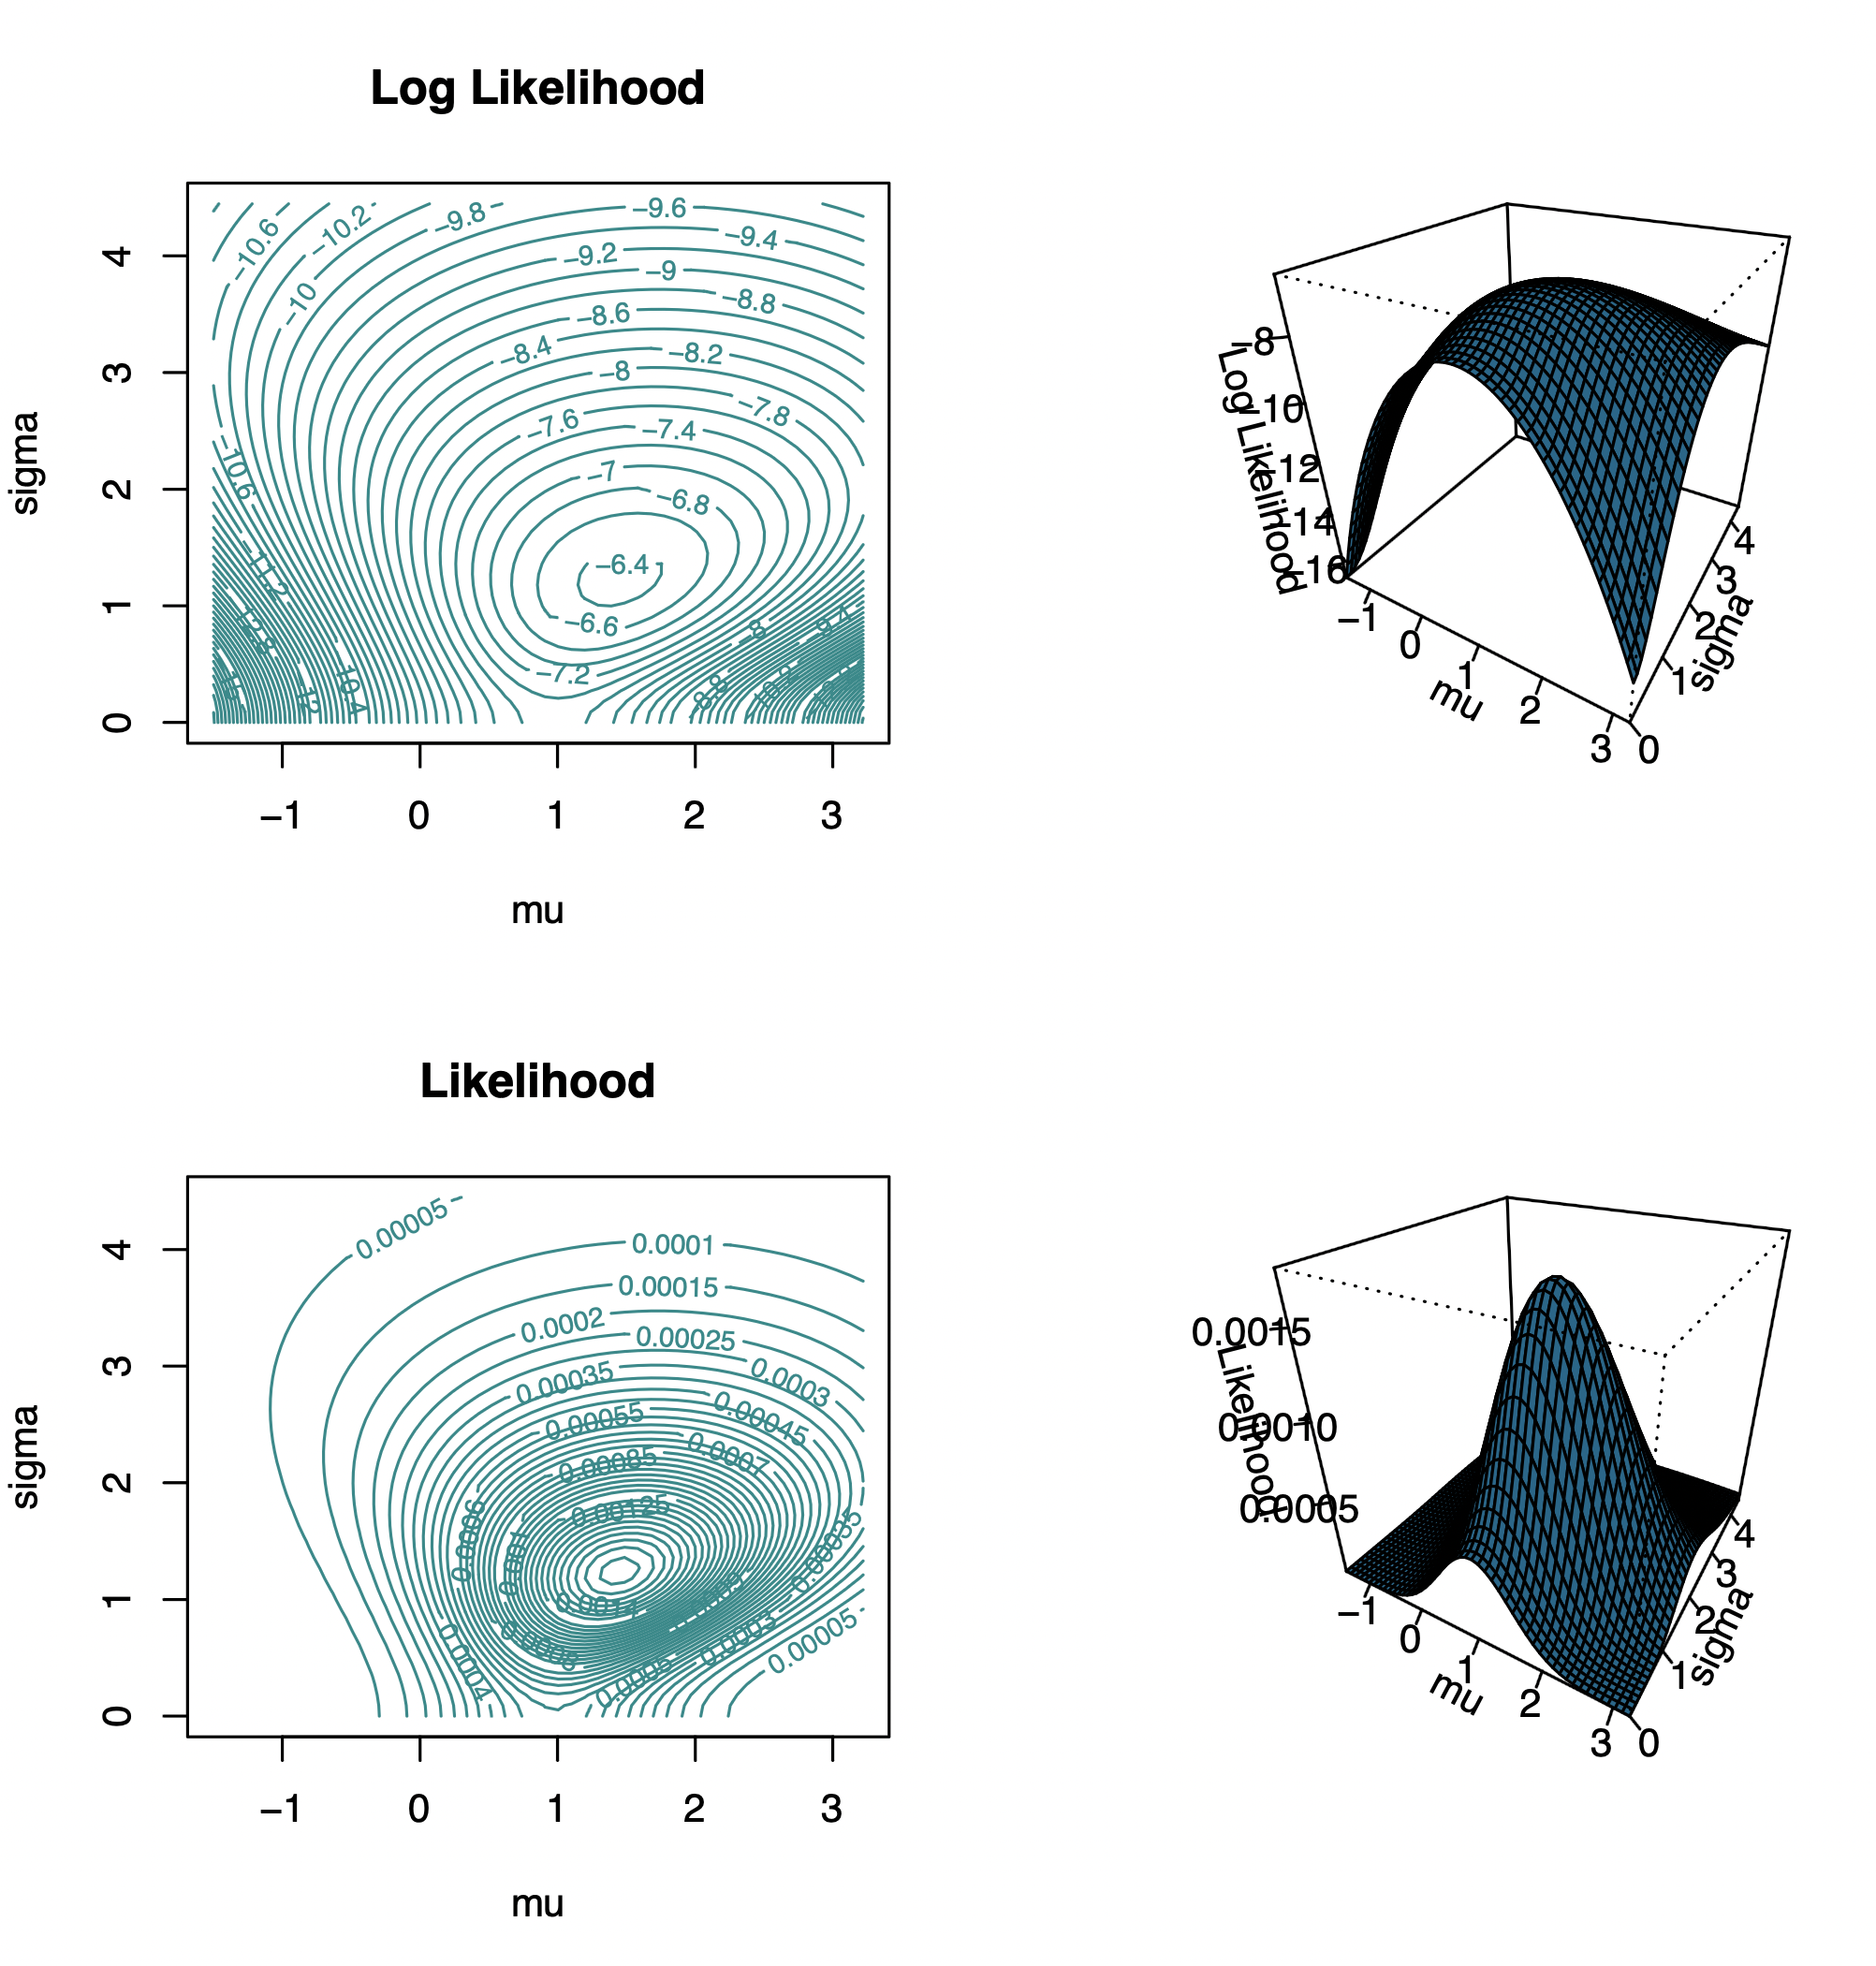
\includegraphics[scale = .45]{2Bc.png}\]
\begin{itemize}

\item[(i)]

With hierarchical data, the concept of \textit{sample size} is trickier than with non-hierarchical data structures: this meta-analysis has a total of $N =$ 10,816 patients but only $k_{ \bm{ \eta } } = 6$ studies. It turns out that the effective sample sizes for $\mu$ and $\sigma$ are driven mainly by $N$ and $k_{ \bm{ \eta } }$, respectively. Do Your plots resemble the large-sample bivariate Normal shapes described above? Explain briefly. \textit{\fbox{\textbf{[5 points]}}}

\begin{solution}
    The log likelihood function does indeed match the what is described above since it has a concave down paraboloid while being a little bit distorted along the $\sigma$ axis. The likelihood function also matches what is described because we see a peak/mountain that looks unimodal with a little bit of distortion like the log likelihood function, but not as much.  
\end{solution}

\item[(ii)]

Does it appear that the likelihood and log-likelihood functions have well-defined unique maxima, at least within the $( \mu, \sigma )$ grid You've used?  Explain briefly. \textit{\fbox{\textbf{[5 points]}}}

\begin{solution}
    Yes, this is because we can clearly see from these graphs that there is no suggestion of multiple maxima, which would suggest multimodality. There is a clear "high" point in both graphs. 
\end{solution}

\end{itemize}

\end{itemize}

In this problem there are two ways to find $\hat{ \bm{ \eta } }$, both of which are useful to know about in contemporary data science, and each of which provides useful information that the other does not:

\begin{itemize}

\item

As we saw in class and in problem 2(A) on this test, when the unknown --- here 
$\bm{ \eta } = ( \mu, \sigma )$ --- has dimension $k_{ \bm{ \eta } } > 1$ and the problem is regular (in the \textit{Exponential-Family} sense), one standard approach to obtain the MLEs, applied to the aspirin meta-analysis, involves (a) creating a system of 2 equations in 2 unknowns by setting each of the first partials with respect to $\mu$ and $\sigma$ equal to 0 and (b) solving for $( \mu, \sigma )$. Sometimes these equations will have closed-form algebraic solutions, but more often in two or more dimensions they have to be solved numerically.

\item

The log-likelihood here is a function $\ell \ell \! \! : \mathbb{ R }^{ k_{ \bm{ \eta }  } } \rightarrow \mathbb{ R }$ that takes as input a vector $\bm{ \eta }$ of real numbers of length $k_{ \bm{ \eta } }$ and returns a real number; such functions can be maximized with general-purpose optimizers. \texttt{R} has a variety of built-in and \texttt{CRAN}--package routines that do this; perhaps the simplest one is the built-in function \texttt{optim}.

\end{itemize}

I've written \texttt{R} code to implement both approaches and posted it in the \texttt{Pages} tab of the course \texttt{Canvas} page; the \texttt{optim} file is called 

\begin{quote}

\texttt{R code for numerical optimization of the log likelihood function} \\ \texttt{for the likelihood analysis in THT 2 problem 2(B)}

\end{quote}

Let's look at how this works, starting with \texttt{optim} first.

\begin{itemize}

%=================================2B - (d) ===================================
\item[(d)]

\textit{\fbox{\textbf{[45 total points for this sub-problem]}}} Download the \texttt{.txt} file just mentiuoned, run my \texttt{optim} code (or an equivalent program in another language), and examine the resulting output (include this output in Your Appendix). 

\begin{itemize}

\item[(i)]

Did the code report convergence to a (local) maximum of the log-likelihood function? \textit{\fbox{\textbf{[5 points]}}} What did the MLE vector turn out to be, to 4 significant figures? \textit{\fbox{\textbf{[5 points]}}} Did the maximum value of $\ell \ell$ agree with what You saw in Your plots in part (c)? \textit{\fbox{\textbf{[5 points]}}} How many function evaluations did \texttt{optim} need to find the MLEs? \textit{\fbox{\textbf{[5 points]}}}

\begin{solution}
    Yes the code reported convergence to a local maximum of the log-likelihood function as can be seen in the appendix from the "\$convergence" output. 

    The MLE vector turned out to be $(1.447, 1.237)$ which is seen from "\$par" output. 

    The maximum value of $\ell\ell$ does agree with our plots. This is because from a quick visual inspection of our plots, the maximum looks to be around (1.5, 1.3). Our code output matches that visual guess. 

    \texttt{optim} needed 43 function evaluations to find the MLE's which can be seen from the "\$counts" ouput under "function". 


\end{solution}

\item[(ii)]

Use the estimated covariance matrix of the MLEs from the \texttt{optim} output to compute estimated standard errors for $\hat{ \mu }_{ MLE }$ and $\hat{ \sigma }_{ MLE }$ (the \textit{hint:} in the \texttt{R} code may help). \textit{\fbox{\textbf{[10 points]}}} \vspace*{0.025in} Since the dose of aspirin in the Treatment group was so low, an excellent clinical argument can be made that the only possibilities for aspirin's effect in these experiments were that aspirin either (I) made no difference or (II) was beneficial in reducing mortality. As we saw in problem 2(A)(d)(i) above, Mr.~Neyman's confidence-interval machinery can be modified to accommodate \textit{one-sided} situations like this: it can be shown (You're not asked to show this) that
\begin{equation} \label{e:lower-confidence-bound-2}
\hat{ \mu }_{ MLE } - \Phi^{ -1 } ( 1 - \alpha ) \cdot \widehat{ SE } \left( \hat{ \mu }_{ MLE } \right)
\end{equation}
is an approximate $100 \, ( 1 - \alpha )$\% \textit{lower confidence bound (LCB)} for $\mu$; in other words, we're $100 ( 1 - \alpha )$\% confident that $\mu$ is \textit{at least} equal to the value in equation (\ref{e:lower-confidence-bound-2}). Compute this LCB for $\alpha = 0.001$. \textit{\fbox{\textbf{[5 points]}}} \vspace*{0.025in} At the 99.9\% level, using maximum likelihood, are we confident that aspirin would indeed reduce mortality for heart-attack patients in the population $\mathcal{ P }$ to which we wish to generalize, based on this meta-analysis? Explain briefly. \textit{\fbox{\textbf{[10 points]}}}

\begin{solution}
    Completing the R code provided in order to computer the estimated standard errors we get (code in appendix), 
    \begin{align*}
        \widehat{SE}(\hat{\mu}_{MLE}) = 0.8394 && \widehat{SE}(\hat{\sigma}_{MLE}) = 0.6791
    \end{align*}

    The LCB for $\alpha = 0.001$ works out to be (using R with the code in appendix) $-1.147494$.
    
    Based on this, we are not confident that aspirin would indeed reduce mortality of heart-attack patients in $\mathcal{P}$. This is because as we see our lower bound is well into the negative region. As discussed in class, under the Devil's Advocate arguement we see the possibility of apsirin doing nothing $(\mu = 0)$ is set inside our confidence interval, making it not Statistically Significant. 
\end{solution}

\end{itemize}

\end{itemize}

Now, as for the method involving setting the first partials of $\ell \ell$ to 0, it can be shown (You're not asked to show this) that one way to express the resulting system of equations with model (\ref{e:random-effects-model}) is
\begin{equation} \label{e:score-equations}
\hat{ \mu } = \frac{ \sum_{ i = 1 }^k \hat{ W }_i \, y_i }{ \sum_{ i = 1 }^k \hat{ W }_i } \ \ \ \textrm{and} \ \ \ \hat{ \sigma }^2 = \frac{ \sum_{ i = 1 }^k \hat{ W }_i^2 \, \left[ ( y_i - \hat{ \mu } )^2 - V_i \right] }{ \sum_{ i = 1 }^k \hat{ W }_i^2 } \, , \ \ \ \textrm{in which} \ \ \ \hat{ W }_i = \frac{ 1 }{ V_i + \hat{ \sigma }^2 } \, .
\end{equation}
As a basis for solving for $( \hat{ \mu }, \hat{ \sigma }^2 )$, this looks odd: the equation for $\hat{ \mu }$ looks okay until You remember that $\hat{ W }_i$ depends on $\hat{ \sigma }^2$, and the equation for $\sigma^2$ is even stranger since it has $\hat{ \sigma }^2$ on both sides (again through $\hat{ W }_i$). However, it turns out that if You \textit{iterate} these equations --- starting with $\hat{ \sigma }^2 = 0$, computing $\hat{ W }_i$, using that to compute $\hat{ \mu }$, using the resulting $\hat{ \mu }$ to compute a new $\hat{ \sigma }^2$, and so on --- they will converge to the MLEs (with one wrinkle: it's possible that $\hat{ \sigma }^2$ may converge to a negative number (!), in which case people avoid embarrassment by setting $\hat{ \sigma }_{ MLE }^2 = 0$). A reasonable convergence criterion involves stopping when two consecutive values of $\hat{ \sigma }^2$ differ by no more than some $\epsilon$ such as $10^{ -7 }$. As part of this technology, there's also a formula for an approximate estimated standard error for $\hat{ \mu }_{ MLE }$:
\begin{equation} \label{e:calibrate-mu-mle}
\widehat{ SE } \left( \hat{ \mu }_{ MLE } \right) = \left[ \sum_{ i = 1 }^k \frac{ 1 }{ V_i + \hat{ \sigma }_{ MLE }^2 } \right]^{ - \frac{ 1 }{ 2 } } \, .
\end{equation}

\begin{itemize}

%============================= 2B - e ===========================================

\item[(e)]

\textit{\fbox{\textbf{[10 total points for this sub-problem]}}} \vspace*{0.025in} \texttt{R} code to implement this algorithm is posted in the \texttt{Pages} tab of the course \texttt{Canvas} page, in a file called

\begin{quote}

\texttt{R code for empirical Bayes calculations in THT 2 problem 2(B)}

\end{quote}

Download this \texttt{.txt} file, run my code (or an equivalent program in another language), and examine the output (include this output in Your Appendix). 

\begin{itemize}
%============================= 2B - e(i) ===========================================
\item[(i)]

How many iterations were needed to achieve convergence with the $\epsilon$ mentioned above? Roughly how much clock time did the algorithm take? \textit{\fbox{\textbf{[5 points]}}}

\begin{solution}
    In order to achieve convergence, 35 iterations were needed. This is seen under the output for "\$m" which is attached in the code appendix. 

    The clock time was roughly about $0.01$ seconds as seen in the output. 
\end{solution}


%============================= 2B - e(ii) ===========================================
\item[(ii)]

Your execution of the code should have produced the following results: $\hat{ \mu }_{ MLE } \doteq 1.447$, with an approximate estimated standard error of $\widehat{ SE } \left( \hat{ \mu }_{ MLE } \right) \doteq 0.8089$, and $( \hat{ \sigma }_{ MLE },$ $\hat{ \sigma }_{ MLE }^2 ) \doteq ( 1.237, 1.531 )$. Bearing in mind (from Table \ref{t:aspirin-case-study-data}) that the typical mortality rate for the control-group patients was about 11\%, would You say that a decline in mortality from taking low-dose aspirin of 1.45 percentage points is large in practical (medical) terms? Would You say that an amount of between-study heterogeneity corresponding to an SD of 1.24 percentage points is large in practical terms? Explain briefly in each case. \textit{\fbox{\textbf{[5 points]}}}
\begin{solution}
    This is definitely large in practical terms, considering the fact that we are talking about life or death and the cost/availability of aspirin (cheap and everywhere basically). Implanting the regular consumption of aspirin in one's life, for a roughly $1.5$ percent decrease in mortality rate, isn't that difficult. Therefore making it practically significant. Another way to see it, is through,
    \[\dfrac{9.55 - 11}{11} = -0.1318 \]
    which means it decreases one's mortality rate by about 13 percent! Which is practical in medical terms. 

    The amount of between-study heterogeneity corresponding to an SD of $1.24\%$ is definitely large in practical terms. This is seen through the large range in mortality rates for the control group between all these studies. Since the control group is being given a placebo, meaning there is no treatment, yet we see substantial differences in their mortality, and our SD of $1.24\%$ captures this. 
\end{solution}
\end{itemize}

\end{itemize}

The maximum-likelihood estimates in this problem are also called \textit{empirical Bayes} estimates, because it turns out that they correspond to a Bayesian analysis in which the prior distribution is to some extent based on the data (this should sound to You like a questionable idea from the Bayesian perspective, because it uses the data both to inform the likelihood function and the prior; it won't surprise You to hear that with small $k$ the result tends to be underpropagation of uncertainty). It can be shown (You're not asked to show this) that the conditional distributions of the random effects $\theta_i$ in model (\ref{e:random-effects-model}) given the data, and also given $\mu$ and $\sigma$, are as follows:
\begin{equation} \label{e:shrinkage-1}
( \theta_i \given y_i \, \mu \, \sigma \, \mathbb{ N } \, \mathcal{ B } ) \stackrel{ \textrm{\footnotesize I} }{ \sim } N \left[ \theta_i^*, V_i ( 1 - B_i ) \right] \, , \ \ \ \textrm{with} \ \ \ \theta_i^* = ( 1 - B_i ) \, y_i + B_i \, \mu \ \ \ \textrm{and} \ \ \ B_i = \frac{ V_i }{ V_i + \sigma^2 } \, .
\end{equation}
In other words, the conditional mean $\theta_i^*$ of the effect for study $i$ given $( y_i,  \mu, \sigma )$ is a weighted average of the sample mean for that study, $y_i$, and the overall mean $\mu$. The weights are given by what are called \textit{shrinkage factors} $B_i$, which in turn depend on how the variability $V_i$ within study $i$ compares to the between-study variability $\sigma^2$: the more accurately $y_i$ estimates $\theta_i$, the more weight the \textit{local} estimate $y_i$ gets in the weighted average (which should make excellent sense to you). The term \textit{shrinkage} refers to the fact that, with this approach, unusually high or low individual studies are drawn back or \textit{shrunken} toward the overall mean $\mu$ when making the calculation $( 1 - B_i ) \, y_i + B_i \, \mu$. Note that $\theta_i^*$ uses data from all the studies to estimate the effect for study $i$: this is referred to as \textit{borrowing strength} in the estimation process, and it also makes excellent sense, because model (\ref{e:random-effects-model}) expresses our scientific judgment that the $k = 6$ studies are similar to each other, which means that there's information in the other $( k - 1 )$ studies when estimating what's going on in study $i$. By functional invariance, the maximum-likelihood estimates of the $B_i$ and $\theta_i$ are
\begin{equation} \label{e:shrinkage-2}
\hat{ B }_i = \frac{ V_i }{ V_i + \hat{ \sigma }^2 } \ \ \ \textrm{and} \ \ \ \hat{ \theta }_i = ( 1 - \hat{ B }_i ) \, y_i + \hat{ B }_i \, \hat{ \mu } \, ,
\end{equation}
and there's an approximate estimated standard error formula for the $\hat{ \theta }_i$:
\begin{equation} \label{e:shrinkage-3}
\widehat{ SE } \left( \hat{ \theta }_i \right) = \sqrt{ V_i \, ( 1 - \hat{ B }_i ) } \, .
\end{equation}

\begin{itemize}

\item[(f)]

\textit{\fbox{\textbf{[30 total points for this sub-problem]}}} \vspace*{0.025in} Use the output from Your previous code execution in part (e) to complete Table \ref{t:mle-results}, and examine the results. In this table, $n_i$ is the combined (Treatment + Control) sample size for study $i$, $p_i = \frac{ n_i }{ \sum_{ j = 1 }^k n_j }$ is the number of patients in study $i$ (expressed as a proportion of the overall number of patients), $\hat{ W }_i^* = \frac{ \hat{ W }_i }{ \sum_{ j = 1 }^k \hat{ W }_j }$ is similarly the $\hat{ W }$ vector normalized to sum to 1 (thus $\hat{ W }_i^*$ is the amount of weight that the data value $y_i$ from study $i$ gets in the weighted average defining $\hat{ \mu }$); the other column headings have already been defined.

\begin{itemize}

\item[(i)]

You can see in equation (\ref{e:shrinkage-2}) that $\hat{ B }_i$ is the amount of weight given to the overall mean $\hat{ \mu }$ in computing the MLE $\hat{ \theta }_i$ for study $i$. One of the points of shrinkage estimation in meta-analysis is to pull outlier studies toward the overall mean, so that they don't overly influence the results. Why is it, then, that study 6 (AMIS), whose $y_i$ is so different from the other $y_i$ values, only gets weight $\hat{ B }_6 \doteq 0.346$ in the computation of $\hat{ \theta }_6$? Explain briefly. \textit{\fbox{\textbf{[10 points]}}}

\begin{solution}
    Well to see this we have to recall the equation for the weight $\hat{B}_i$ is determined,
    \[\hat{B_i} = \dfrac{V_i}{V_i + \hat{\sigma}^{2}}\]
    meaning if a sample has a low $V_i$ the value of its $\hat{B_i}$ will also be low (because the numerator would be small). We see from the table that study 6 has the lowest $V_i$, which is due from it having the largest sample size, so therefore it must have the lowest $\hat{B_i}$ weight, even though its $y_i$ is the most different from the rest. 
\end{solution}

\item[(ii)]

Compare the $p_i$ and $\hat{ W }_i^*$ columns in Table \ref{t:mle-results}. How do You explain the fact that study 6 (AMIS) had about 42\% of the total number of patients but only got 28\% of the total weight in computing $\hat{ \mu }$? \textit{\fbox{\textbf{[10 points]}}}

\begin{solution}
    Like before, this can explained by seeing how we determined $\hat{W_i}^{*}$ which we know from (22) to be calculated by,
    \[\hat{W_i}^{*} = \dfrac{1}{V_i + \hat{\sigma}^{2}}.\]
    So, while it is true that study 6 has the smallest $V_i$, it doesn't change the fact that $\sigma^{2}$ is large, which will make the result of the fraction small. This is because $\sigma^{2}$ represents the between-study heterogeneity, which is high in this meta-analysis, and study 6 actually plays a big role in making it large. 
\end{solution}

\item[(iii)]

Compute the unweighted average of the $\hat{ \theta }_i$ values in Table \ref{t:mle-results}. How, if at all, does the result relate to Your other maximum-likelihood estimation findings? Is what You've just found sensible? Explain briefly. \textit{\fbox{\textbf{[10 points]}}}
\begin{solution}
    Looking at the output of our code in the appendix, under "\$theta.hat" we see these values relate to the maximum-likelihood estimation through the fact that,
    \[\dfrac{1}{k}\sum_{i = 1}^{k}\hat{\theta_i} = \hat{\mu}.\]
    This is because the $\theta_i$ values are drawn from a normal curve with a mean $\mu$, which we see in the middle line of equation (17). So for this line to be consistent and true, the relation above must be true.  
\end{solution}
\end{itemize}

\end{itemize}

\begin{table}[t!]

\centering

\caption{\textit{Maximum-likelihood empirical Bayes results in the aspirin meta-analysis. The symbols in the column headings are explained in the text.}}

\label{t:mle-results}

\bigskip

\begin{tabular}{c|rlclcrrl}

Study $( i )$ & \multicolumn{1}{c}{$n_i$} & \multicolumn{1}{c}{$p_i$} & $\hat{ W }_i$ & \multicolumn{1}{c}{$\hat{ W }_i^*$} & $\hat{ B }_i$ & \multicolumn{1}{c}{$y_i$} & \multicolumn{1}{c}{$\hat{ \theta }_i$} & \multicolumn{1}{c}{$\widehat{ SE } \! \left( \hat{ \theta }_i \right)$}\\

\hline

1 & 1239 & 0.115 & 0.235 & 0.154 & 0.640 & $\tcr{2.77}$ & $\tcr{1.92}$& 0.990 \\

2 & $\tcr{1529}$& 0.141 & $\tcr{0.308}$ & 0.202 & 0.529 & 2.50 & 1.94 & 0.899 \\

3 & 626 & 0.0579 &$\tcr{0.143}$ & 0.0934 & 0.782 & 1.84 & 1.53 & $\tcr{1.09}$\\

4 & 1682 & $\tcr{0.156}$ & 0.232 & $\tcr{0.152}$& 0.646 & 2.56 & 1.84 & 0.994 \\

5 & $\tcr{1216}$& 0.112 & 0.183 & 0.120 & 0.719 &$\tcr{2.32}$ & $\tcr{1.69}$& 1.04 \\

6 & 4524 & $\tcr{0.418}$& 0.427 & 0.280 & 0.346 & $-1.15$ & $-0.251$ & $\tcr{0.728}$

\end{tabular}

\end{table}

In the rest of this problem You'll perform a Bayesian analysis of the data in Table \ref{t:aspirin-case-study-data}. Looking back at equation (\ref{e:random-effects-model}), the second and third rows of the hierarchical model are the same as in the maximum-likelihood approach, but we now need to specify a prior distribution for $( \mu, \sigma )$. The meta-analysis summarized by Table \ref{t:aspirin-case-study-data} was the first of its kind, so we want to build a low-information (LI, otherwise known as \textit{diffuse}) prior. There is no conjugate prior for this situation; we need to use MCMC to quantify the posterior.

It turns out that there is typically little harm in treating $\mu$ and $\sigma$ as independent in constructing $p ( \mu \, \sigma \given \mathcal{ B } )$ (whatever dependence they should have in the posterior will be imposed by the likelihood), so let's use a prior of the form $p ( \mu \, \sigma \given \mathcal{ B } ) = p ( \mu \given \mathcal{ B } ) \cdot p ( \sigma \given \mathcal{ B } )$. There are a number of ways to make this prior diffuse; research has shown two things: 

\begin{itemize}

\item

The posterior is insensitive to the precise details specifying $p ( \mu \given \mathcal{ B } )$ as long as it's close to flat in the region where the likelihood is appreciable, so let's use a prior of the form $( \mu \given \mathcal{ B } ) \sim \textrm{Uniform} ( A, B )$, where $A$ and $B$ are chosen to avoid inappropriate truncation of the posterior; and

\item

Care \bi{is} required in specifying $p ( \sigma \given \mathcal{ B } )$ diffusely to achieve good calibration, especially when $k$ is small (which it is here). The consensus of the research on this topic is that a well-calibrated choice that achieves a diffuse prior on $\sigma$ is $( \sigma \given \mathcal{ B } ) \sim \textrm{Uniform} ( 0, C )$, where $C$ is chosen large enough to again avoid truncation of the posterior (but not much larger than that). 

\end{itemize}

I've written \texttt{rjags} and other \texttt{R} code so that You can do the MCMC computations in this case study, and posted it on the \texttt{Pages} tab of the course \texttt{Canvas} page; the file is called
\begin{quote}

\texttt{rjags and other R code for MCMC calculations in THT 2 problem 2(B)}

\end{quote}
After some experimentation I chose $( A, B, C ) = ( -2, 5, 6 )$ in the prior specification. Download the \texttt{.txt} file just mentioned, run parts (0)--(11) of my code (or an equivalent program in some other language), stopping at each place where stopping is suggested, and examine the output; make PDF files of all plots the code produces and include them in Your solutions.

\begin{table}[t!]

\centering

\caption{\textit{Maximum-likelihood and Bayesian results in the aspirin meta-analysis; --- means that results with the indicated method for the indicated quantity are not available.}}

\label{t:ml-bayes-comparison}

\bigskip

\begin{tabular}{c||ccc|ccl}

\multicolumn{1}{c}{} & \multicolumn{3}{c}{Maximum-Likelihood} & & \multicolumn{2}{c}{Bayesian} \\ \cline{2-4}

\multicolumn{1}{c}{} & & \multicolumn{2}{c}{Standard Error} & & \multicolumn{2}{c}{Posterior} \\ \cline{3-4} \cline{6-7}

\multicolumn{1}{c}{Quantity} & Estimate & Information-Based & \multicolumn{1}{c}{Empirical Bayes} & & Mean & \multicolumn{1}{c}{SD} \\

\hline

$\mu$ & \ 1.447 & 0.8394 & \ 0.8089 & & \ 1.502 & 1.056 \\

$\sigma$ & \ 1.237 & 0.6791 & --- & & \ 1.896 & 1.079 \\

$\theta_1$ & \ 1.923 & --- & \ 0.9899 & &\  $\tcr{2.096}$ & $\tcr{1.319}$\\

$\theta_2$ &\ $\tcr{1.943}$ & --- & \ 0.8995 & & \ 2.042 & $\tcr{1.130}$ \\

$\theta_3$ & \ 1.533 & --- &$\tcr{1.094}$ & & \ 1.592 & 1.542 \\

$\theta_4$ & \ 1.841 & --- & \ 0.9941 & &\ $\tcr{1.984}$ & 1.315 \\

$\theta_5$ &\ $\tcr{1.692}$ & --- & 1.049 & & \ 1.812 & 1.431 \\

$\theta_6$ & $-0.2514$ & --- & \ 0.7278 & & $-0.4327$ & 0.9425 \\

\end{tabular}

\end{table}

\begin{itemize}
%=================== Problem g ============================
\item[(g)]

\textit{\fbox{\textbf{[60 total points for this sub-problem]}}} \vspace*{0.025in} Use the output from Your MCMC code execution to complete Table \ref{t:ml-bayes-comparison} by filling in the blank entries; answering the questions below will also involve extracting additional numbers from the output.
\begin{tcolorbox}
    The plots and the code output during my execution will be in the code appendix. 
\end{tcolorbox}
\begin{itemize}

\item[(i)]

Compare the posterior mean for $\mu$ with its maximum-likelihood (ML) counterpart; then compare the posterior SD for $\mu$ with the two ML standard errors, one likelihood-based and the other from empirical Bayes considerations.  \textit{\fbox{\textbf{[10 points]}}} \vspace*{0.025in} Research on hierarchical models with random effects, such as model (\ref{e:random-effects-model}), has shown that Bayes and ML findings will either be similar (when $k$ is large) or the ML approach will often underestimate uncertainty when it differs from Bayes. Does the second of those two possibilities appear to have happened here? Explain briefly. \fbox{\textbf{\textit{[5 points]}}}
\begin{solution}
    Well from our table we see that the pertenage points of mortality reduction for the posterior mean $\mu$ is about $1.502$ and under ML it is about $1.447$. Which are somehwat close to each other.
    
    The posterior standard deviation for $\mu$ is about $1.056$, and the under ML, information based standard error is $0.8394$ and the emperical bayes is  $0.8089$. Here we see a bigger difference, under ML we have less uncertainty compared to the posterior uncertainty. 

    We see from our comparision that the second case is happening here, since our $k$ is only 6, and the ML approach is underestimating our uncertainty compared to Bayes. Since our uncertainty under Bayes is about $1.056$ which is considerably larger than  $0.8394$ and $0.8089$. Meaning Bayes provides a better SD than ML since it is an underestimate due to the small $k$.
    
\end{solution}

\item[(ii)]

Compare the posterior mean for $\sigma$ with its ML counterpart; are they close enough that it doesn't matter which one You would report in a research article or white paper for a client? \textit{\fbox{\textbf{[10 points]}}} Extract the 99.9\% Bayesian posterior interval for $\sigma$ from the output and report it here. \textit{\fbox{\textbf{[5 points]}}} Compute the large-sample-approximate 99.9\% confidence interval for $\sigma$ from maximum-likelihood, thereby showing that it has embarrassed itself by going negative. \textit{\fbox{\textbf{[5 points]}}} \vspace*{0.025in} Focusing on the Bayesian interval, if the Devil's Advocate (let's say female, to have a pronoun) said to You, ``I think that $\sigma$ is actually 0 in the population of \{randomized controlled trials that could have been run in the late 1980s in Europe and the U.S.~to compare aspirin with placebo for patients who have had a heart attack\}, and the only reason You got something different from 0 was that the 6 studies in Your meta-analysis were unlucky,'' would You agree with her? Does this mean that $\sigma$ is statistically significantly different from 0? Explain briefly. \textit{\fbox{\textbf{[10 points]}}}

\begin{solution}
    We see the posterior mean for $\sigma$ to be $1.896$ and the ML mean for $\sigma$ is $1.237$. We see that the posterior mean for $\sigma$ is about 50 percent larger than the ML mean for $\sigma$. It is clear from this that it certaintly matters which one we choose to report, due to the substantial difference.

    From the code provided we see our 99.9\% Bayesian posterior interval for $\sigma$ is:
    \[(0.002, 5.94)\]

    Now calculating the large-sample-approximate 99.9\% CI for $\sigma$ from the maximum-likelihood is simply,
    \begin{align*}
        1.237 \pm \Phi^{-1}\lrp{1 - \dfrac{\alpha}{2}}0.6791 = 1.237 \pm 3.29 \cdot 0.6791 = (-1.0, 3.5)
    \end{align*}
    which is well into the negative region. 

    We wouldn't agree with her here because we can see that 0 is not in our 99.9\% Bayesian confidence interval, meaning that $\sigma$ is statistically significant from 0 at this level of confidence based on the data. 


\end{solution}

\item[(iii)]

Show (by extracting the relevant number from Your output) that, conditional on model (\ref{e:random-effects-model}) and the prior used to produce Your output, the posterior probability that low-dose aspirin would be beneficial, if used in the population $\mathcal{ P }$ identified just above item (a) in this problem, is about 93\%. \textit{\fbox{\textbf{[5 points]}}} \vspace*{0.025in} Is this standard of envidence strong enough for You personally to recommend the use of low-dose aspirin to prevent future heart attacks and strokes in $\mathcal{ P }$? Briefly explain Your reasoning. (There is no single right answer to this question.) \textit{\fbox{\textbf{[10 points]}}}
\begin{solution}
    We see that the probability of $\mu$ being positive (beneficial) when conditioning on the data, the low information prior, model 17, and the background, we get it to be about 0.9332 or about 93\% as desired.

    Under today's standards of replicability no, but personally I would recommend it if one is willing, but only to the people like the ones in studies 1-5. This is because for the people of study 6, aspirin was not found to be helpeful at all. The reason I would recommend it, if people woudld like, is because the cost and side effects of taking aspirin are not large or worrying, so for the potential gain that may be recieved (not dying) it may be worth it. I definitely wouldn't strongly advise it or recommend to make it some sort of standard treatment based on this though. 
\end{solution}
\end{itemize}


\item[(h)]

\textit{\fbox{\textbf{[20 total points for this sub-problem]}}} \vspace*{0.025in} Finally, let's make a formal comparison of the ran\-dom-effects model (studied above in the rest of this problem) with the following \textit{fixed-effects} model for $( i = 1, \dots, k )$:
\begin{eqnarray} \label{e:fixed-effects-model}
( \mu \given \mathcal{ B } ) & \sim & p ( \mu \given \mathcal{ B } ) \nonumber \\
( y_i \given \mu \, V_i \, \mathcal{ B } ) & \stackrel{ \textrm{\footnotesize IID} }{ \sim } & N ( \mu, V_i ) \, .
\end{eqnarray}
We'll be using the Bayesian model comparison method called \textit{DIC} (the \textit{Deviance Information Criterion}), discussed in class as one of several such methods (and one that's suitable for working with random effects models); in \texttt{rjags} \textit{DIC} is referred to as the \textit{penalized deviance}.
\begin{tcolorbox}
    The plot and code output will be in the code appendix. 
\end{tcolorbox}
\begin{itemize}

\item[(i)]

By examining the random effects model equations (\ref{e:random-effects-model}), briefly explain why the fixed effects model in (\ref{e:fixed-effects-model}) is a special case of (\ref{e:random-effects-model}) in which it's assumed that $\sigma = 0$. \textit{\fbox{\textbf{[5 points]}}}

\begin{solution}
    Well $\sigma$ is representing our between-study heterogeneity, so if $\sigma$ were to be 0, our middle layer in modle (17) will dissapear since all the $\theta_i$'s would be deterministically equal to $\mu$ (because a Normal distribution with mean $\mu$ and variance 0 would be a point mass at $\mu$). Meaning we would only need a prior for $\mu$, giving us model (27). Therefore model (27) is a special case of model (17) where $\sigma = 0$. 
\end{solution}

\item[(ii)]

Run the final block of code (section (12) in the \texttt{rjags} code file) to get 
\textit{DIC} values for the fixed effects and random effects models. Use your output to fill in the missing (blank) entries in Table \ref{t:dic-comparison}. Bearing in mind that \textit{DIC} is set up so that smaller values indicate better models, which of the two models is more strongly supported by the \textit{DIC} evidence here? Does this agree with your conclusions about between-study heterogeneity in the earlier parts of this problem? Explain briefly. \textit{\fbox{\textbf{[15 points]}}}

\begin{solution}
    It is clear that the random effects models is better than fixed effect models. It is difficult to say if this differene is enough though to \textit{strongly} suggest it over fixed effects. What we can say is that random effect models is better here, but we can't say how much better based on this difference. This does agree with our conclusions of between-study heterogeneity since using the model that takes it into account turned out to be better than assuming there to be none. So our suspicion of between-study heterogeneity turned out to be correct. 
\end{solution}

\end{itemize}

\begin{table}[t!]

\centering

\caption{\textit{DIC comparison of the fixed effects and random effects models in the aspirin meta-analysis.}}

\label{t:dic-comparison}

\bigskip

\begin{tabular}{c|ccc}

& Mean & Complexity \\
Model & Deviance & Penalty & \textit{DIC} \\

\hline

Fixed Effects & $\tcr{27.1 }$& 1.0 &  $\tcr{28.1}$\\
Random Effects & 21.6 & $\tcr{4.1}$& 25.7

\end{tabular}

\end{table}

\vspace*{3.0in}

\end{itemize}

\newpage

\textbf{CODE FOR PROBLEMS}
Apart from the the code explicitly given to use for certain problems, a lot of this code taken or influenced from the office hours given by professor Draper. 

\tcr{$\bm{START ==== 2A - di (Method 1) =========================}$}
\begin{lstlisting}[language = R]
n.1 <- 659 #Biden
n.2 <- 554 #Trump
n.3 <- 52 #Other

n <- n.1 + n.2 + n.3 #Total sample

                    #Proportions
theta.1 <- n.1 / n  #Biden
theta.2 <- n.2 / n  #Trump
theta.3 <- n.3 / n  #Other

gamma <- theta.1 - theta.2

#Variances of theta.1, theta.2 and theta.3
SE.hat.theta.1 = sqrt((theta.1 * (1 - theta.1) )/n )
SE.hat.theta.2 = sqrt((theta.2 * (1 - theta.2) )/n )
SE.hat.theta.3 = sqrt((theta.3 * (1 - theta.3) )/n )

estimated.variance.gamma <- (theta.1 * (1-theta.1)/n) + 
    (theta.2 * (1-theta.2)/n) + 2*( (theta.1 * theta.2)/ n)

SE.hat.gamma <- sqrt(estimated.variance.gamma)

print(estimated.variance.gamma)
print(SE.hat.gamma)

print(theta.1)
print(theta.2)
print(theta.3)
\end{lstlisting}
\tcr{$\bm{END ==== 2A - di (Method 1) =========================}$}

\vspace*{1in}
\tcr{$\bm{START ======= 2A - f (ii) ==========================}$}
\begin{lstlisting}[language = R]
options(scipen=999)
rdirichlet <- function( M, alpha ) {
  k <- length( alpha )
  theta.star <- matrix( NA, M, k )
  for ( j in 1:k ) {
    theta.star[ , j ] <- rgamma( M, alpha[ j ], 1 )
  }
  theta.star <- theta.star / apply( theta.star, 1, sum )
  return( theta.star )
}

epsilon <- 0.01
k <- 3
alpha.prior <- rep(epsilon, k)

n.1 <- 659 #Biden
n.2 <- 554 #Trump
n.3 <- 52 #Other

n <- c(n.1, n.2 , n.3) 

alpha.posterior <- alpha.prior + n
 
M.0 <- 100000 #pilot M
str(
  initial.MC.data.set <- rdirichlet(M.0, alpha.posterior)
)

initial.MC.posterior.mean.estimates <-apply(initial.MC.data.set, 2, mean)

initial.MC.posterior.sd.estimates <- apply(initial.MC.data.set, 2, sd)

theta.1.star <- initial.MC.data.set[, 1]
theta.2.star <- initial.MC.data.set[, 2]
theta.3.star <- initial.MC.data.set[, 3]

gamma.star <- theta.1.star - theta.2.star

initial.MC.data.set.gamma.star <- cbind(theta.1.star, 
    theta.2.star, theta.3.star, gamma.star)


#Standard error of each theta_i
mcse.theta.1.bar.star <- sd(theta.1.star)/ sqrt(M.0)
mcse.theta.2.bar.star <- sd(theta.2.star)/ sqrt(M.0)
mcse.theta.3.bar.star <- sd(theta.3.star)/ sqrt(M.0)

gamma.star.mean <- mean(gamma.star)

#Standard Error of gamma
mcse.gmma.bar.star <- sd(gamma.star) / sqrt(M.0)

#The needed M which we use next
needed.M.0 <- ceiling((sd(gamma.star)/ 0.00005)^2)
\end{lstlisting}

\tcr{$\bm{\text{START OF USING UPDATED M VALUE}  ============}$}

\begin{lstlisting}
M.0 <- needed.M.0 #updated M
str(
  final.MC.data.set <- rdirichlet(M.0, alpha.posterior)
)

final.MC.posterior.mean.estimates <-apply(final.MC.data.set, 2, mean)

final.MC.posterior.sd.estimates <- apply(final.MC.data.set, 2, sd)

theta.1.star <- final.MC.data.set[, 1]
theta.2.star <- final.MC.data.set[, 2]
theta.3.star <- final.MC.data.set[, 3]

gamma.star <- theta.1.star - theta.2.star

final.MC.data.set.gamma.star <- cbind(theta.1.star, 
    theta.2.star, theta.3.star, gamma.star)


mcse.theta.1.bar.star <- sd(theta.1.star)/ sqrt(M.0)
mcse.theta.2.bar.star <- sd(theta.2.star)/ sqrt(M.0)
mcse.theta.3.bar.star <- sd(theta.3.star)/ sqrt(M.0)

mcse.gmma.bar.star <- sd(gamma.star) / sqrt(M.0)
\end{lstlisting}
\tcr{$\bm{END ======= 2A - f(ii) =====================}$}
\vspace*{1in}

\tcr{$\bm{START ===== 2A - f(v)========}$}
\begin{lstlisting}[language = R]
#This is the code that gave the values,
#but it uses the code right above
print(mean(gamma.star > 0))
print(sd(gamma.star > 0)/ sqrt(M.0))
\end{lstlisting}
\tcr{$\bm{END ===== 2A - f(v)========}$}

\vspace*{1in}

\tcr{$\bm{START ==== 2B - c(i) \& c(ii) =====================}$}
\begin{lstlisting}[language = R]

#Used R file provided to us on canvas to generate graphs

\end{lstlisting}
\tcr{$\bm{END ====== 2B - c(i) \& c(ii)====================}$}

\vspace*{1in}
\tcr{$\bm{START ===== 2B - d(i) ============================}$}
\begin{lstlisting}[language = R]
#This is code given to us, but I deleted all the comments due to length
# enter the data:

y <- c( 2.77, 2.50, 1.84, 2.56, 2.32, -1.15 )
V <- c( 1.65, 1.31, 2.34, 1.67, 1.98, 0.90 )^2

aspirin.mortality.log.likelihood.for.optim <- function( eta, y, V ) {
  mu <- eta[ 1 ]
  sigma <- eta[ 2 ]
  ll <- ( - 1 / 2 ) * sum( log( V + sigma^2 ) + ( y - mu )^2 /
                             ( V + sigma^2 ) )
  return( ll )
} 

eta.initial.values <- c( 1.5, 1.25 )
print( ml.results.1 <- optim( eta.initial.values, 
                        aspirin.mortality.log.likelihood.for.optim, 
                        y = y, V = V, 
                        hessian = T, control = list( fnscale = -1 ) ) )

print( maximum.likelihood.covariance.matrix <- 
         solve( - ml.results.1$hessian ) )

print( 
    maximum.likelihood.estimated.standard.errors <- 
        diag(maximum.likelihood.covariance.matrix)  
    )
    
#OUTPUT
#$par
#[1] 1.446576 1.237251

#$value
#[1] -6.332311

#$counts
#function gradient 
#      43       NA 

#$convergence
#[1] 0

#$message
#NULL

#$hessian
#           [,1]       [,2]
#[1,] -1.5279769  0.5041351
#[2,]  0.5041351 -2.3347060

#          [,1]      [,2]
#[1,] 0.7046628 0.1521584
#[2,] 0.1521584 0.4611751
#[1] 0.8394419 0.6790988   
\end{lstlisting}
\tcr{$\bm{END ===== 2B - d(i) ============================}$}
\vspace*{1in}

\tcr{$\bm{START ====== 2B - d(ii) =======================} $}
\begin{lstlisting}[language = R]
alpha <- 0.001

print(1.446576 - qnorm(1 - alpha) * 0.8394419)
\end{lstlisting}
\tcr{$\bm{END ===== 2B - d(ii) ========================}$}
\vspace*{1in}

\tcr{$\bm{START ===== 2B - e(i)(ii)(iii)========================}$}
\begin{lstlisting}[language = R]
#Used the code provided from the .txt file mentioned in the 
#problem statement
#When ran this is the OUTPUT
$m
[1] 35

$mu.hat
[1] 1.446869

$se.hat.mu.hat
[1] 0.8089829

$sigma.squared.hat
[1] 1.530753

$sigma.hat
[1] 1.237236

$n
[1] 1239 1529  626 1682 1216 4524

$n.normalized
[1] 0.11455251 0.14136464 0.05787722 0.15551036 0.11242604 0.41826923

$W.hat
[1] 0.2351142 0.3079905 0.1427276 0.2315001 0.1834474 0.4272130

$W.hat.normalized
[1] 0.15387125 0.20156544 0.09340856 0.15150600 0.12005779 0.27959095

$B.hat
[1] 0.6400983 0.5285426 0.7815193 0.6456306 0.7191873 0.3460425

$y
[1]  2.77  2.50  1.84  2.56  2.32 -1.15

$theta.hat
[1]  1.9230658  1.9433752  1.5327602  1.8413283  1.6920550 -0.2513731

$se.hat.theta.hat
[1] 0.9898648 0.8994821 1.0937609 0.9941332 1.0492369 0.7278087

   user  system elapsed 
  0.011   0.000   0.011     
\end{lstlisting}
\tcr{$\bm{END ===== 2B - e(i)(ii)(iii)========================}$}

\vspace*{1in}
\tcr{$\bm{START ======= 2B - g(i)(ii)(iii)======================}$}
\begin{lstlisting}
#Code used was provided, I didn't modify it other than to print values
#so I won't be pasting it here to save space
#CODE OUTPUT    
Compiling model graph
   Resolving undeclared variables
   Allocating nodes
Graph information:
   Observed stochastic nodes: 6
   Unobserved stochastic nodes: 8
   Total graph size: 30

Initializing model

  |++++++++++++++++++++++++++++++++++++++++++++++++++| 100%
  |**************************************************| 100%
  |**************************************************| 100%
[1] 0.567431
[1] 0.006355817
                        0.05%    99.95% 
1.8874320 1.0879348 0.0105058 5.9327306 
[1] 0.7766925
[1] 0.009704146
 'mcarray' num [1:6, 1:100000, 1] 2.95 1.76 3.77 3.35 3.52 ...
 - attr(*, "varname")= chr "theta"
 - attr(*, "type")= chr "trace"
 - attr(*, "iterations")= Named num [1:3] 2001 102000 1
  ..- attr(*, "names")= chr [1:3] "start" "end" "thin"
[1]  2.0957896  2.0390408  1.5898098  1.9838042  1.8203684 -0.4211204
[1] 1.318550 1.129905 1.535767 1.316264 1.431770 0.951049
[1] 0.93344
\end{lstlisting}


\vspace*{1in}

\[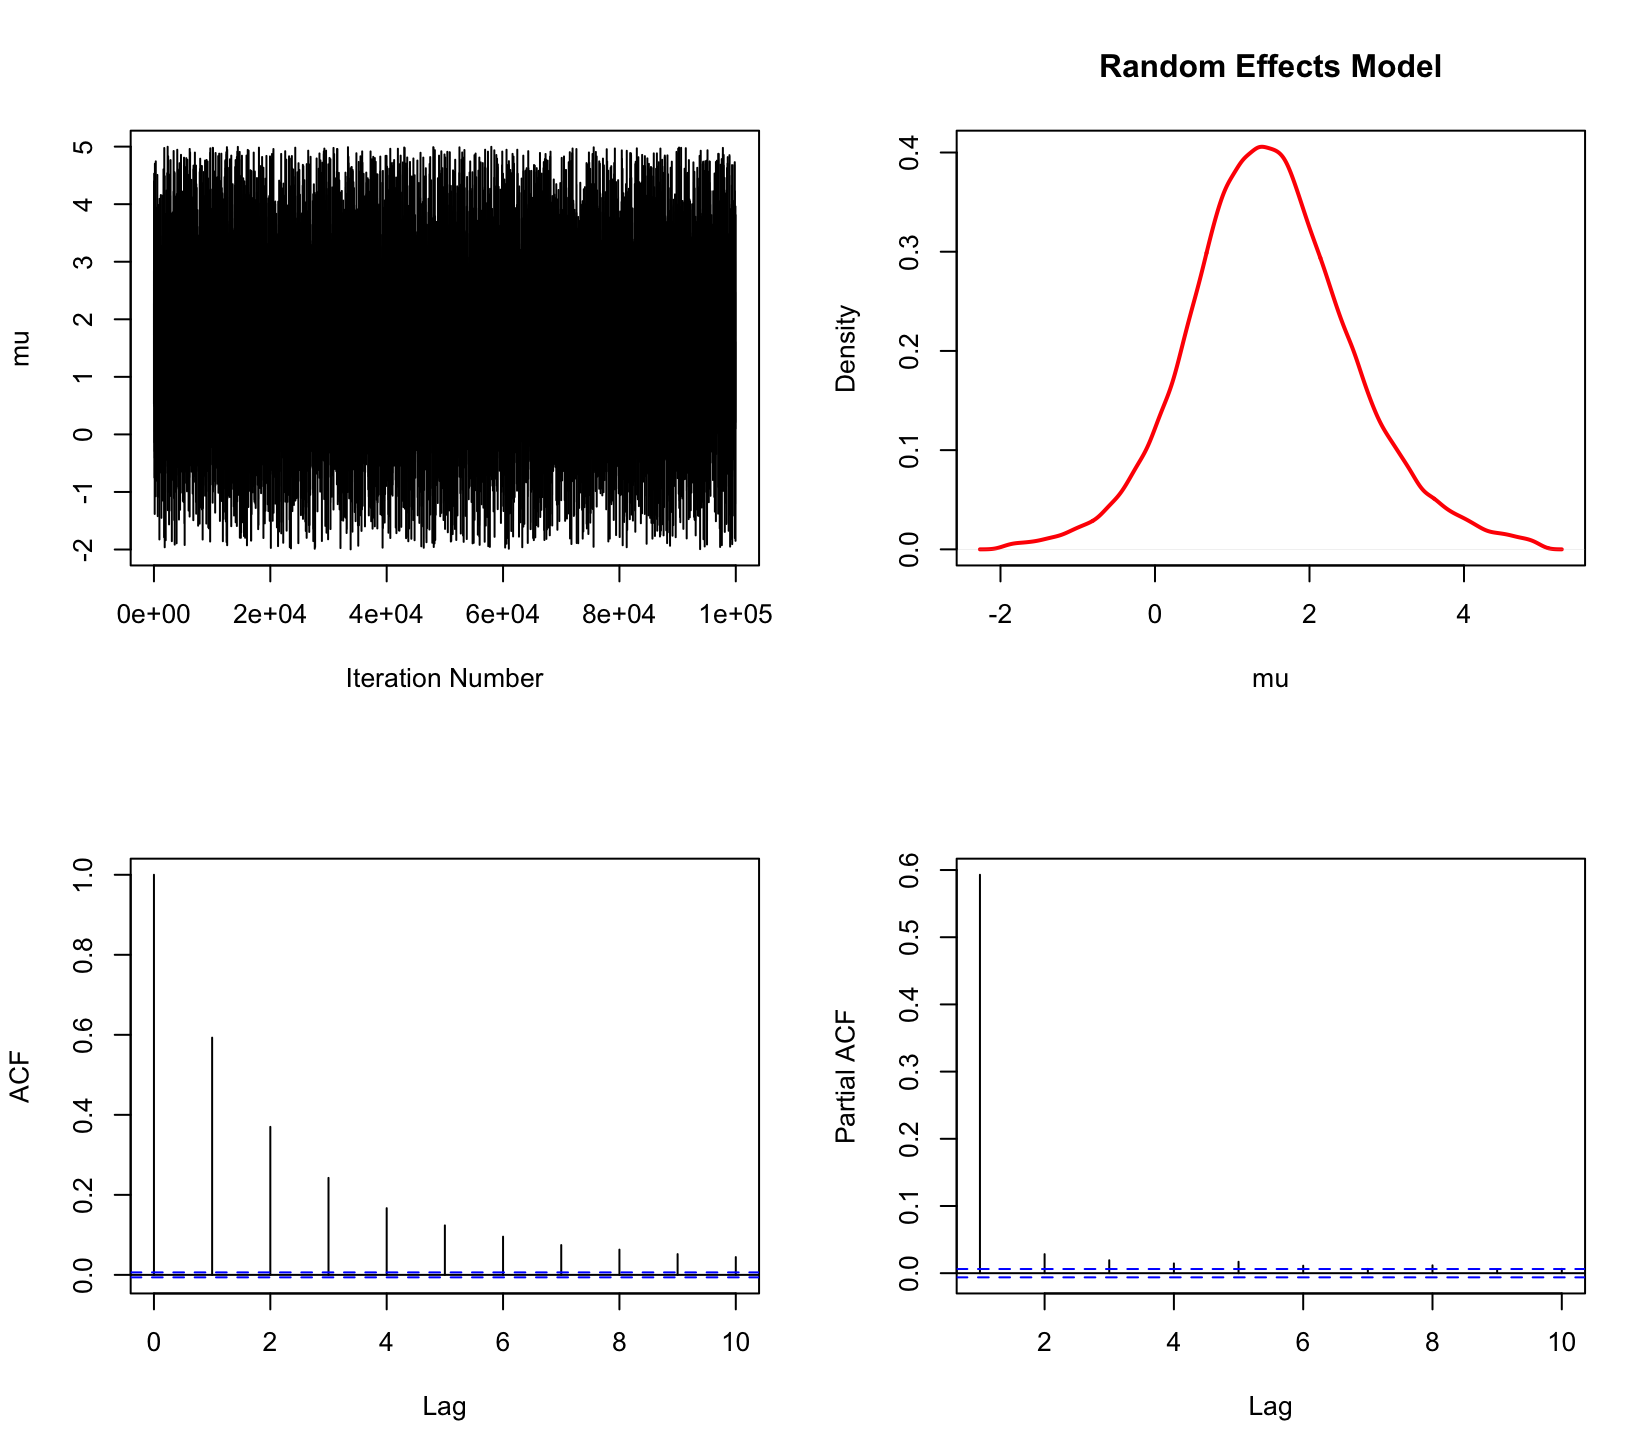
\includegraphics[scale = .3]{2Bg1.png}\]

\[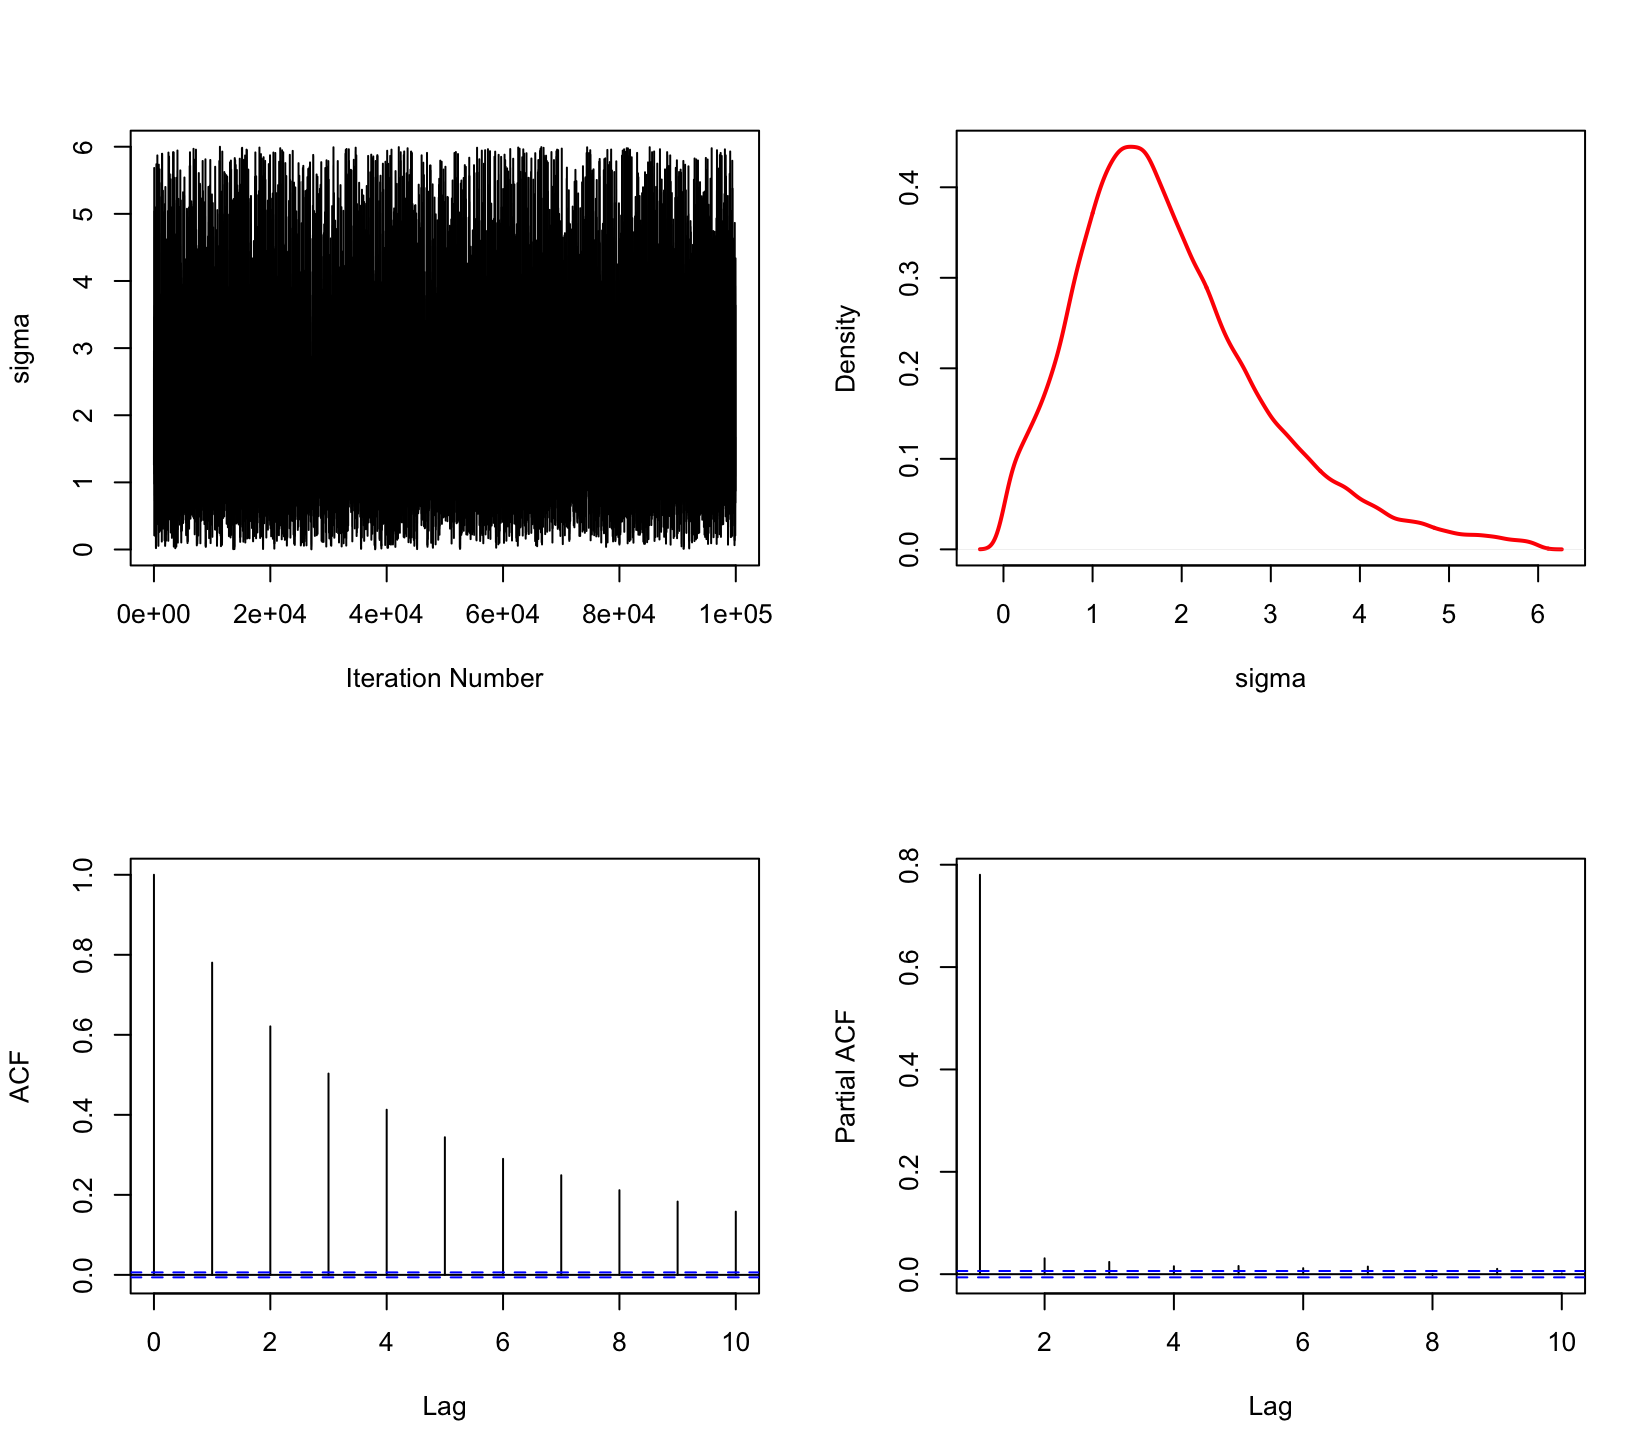
\includegraphics[scale = .3]{2Bg2.png}\]

\[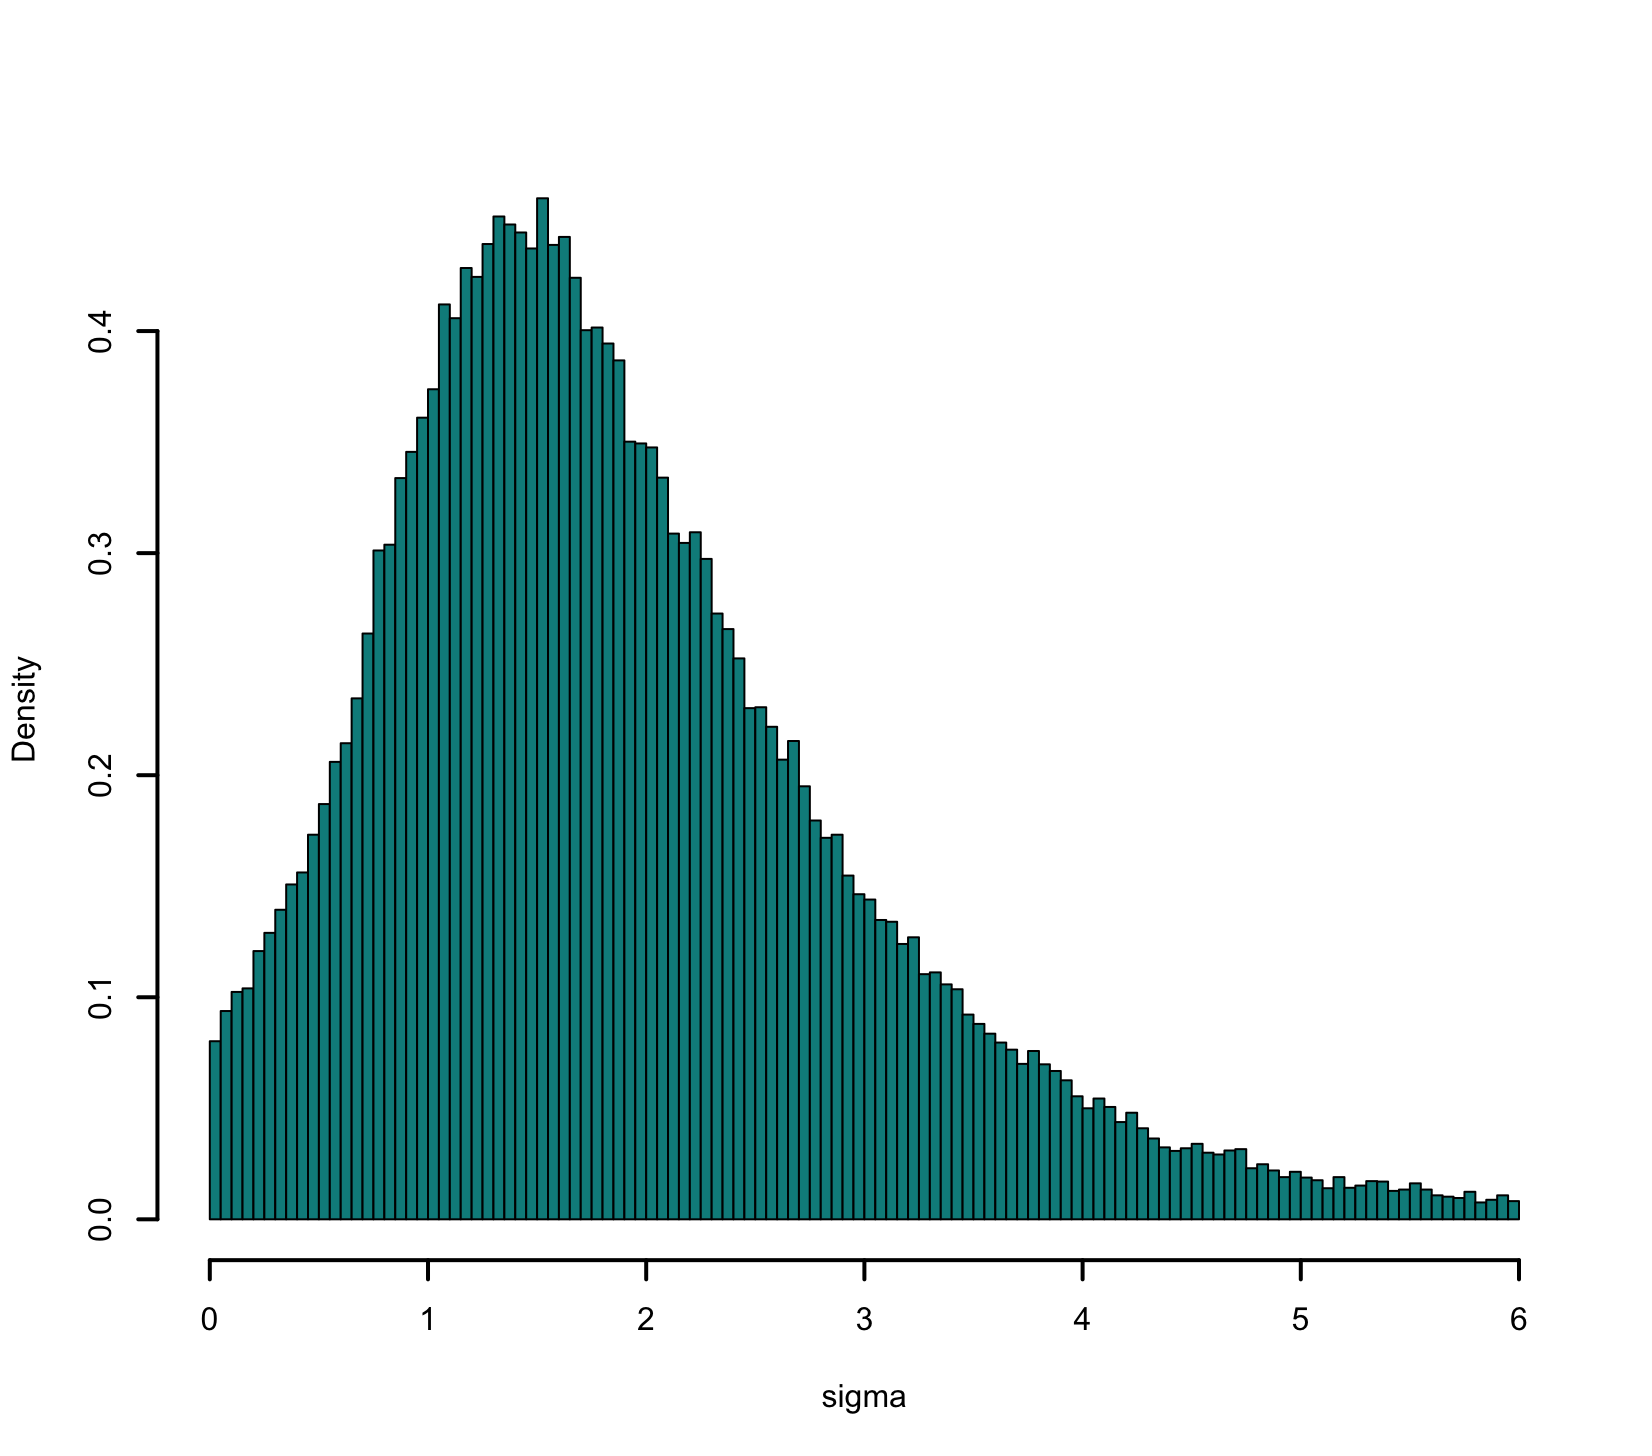
\includegraphics[scale = .3]{2Bg3.png}\]

\[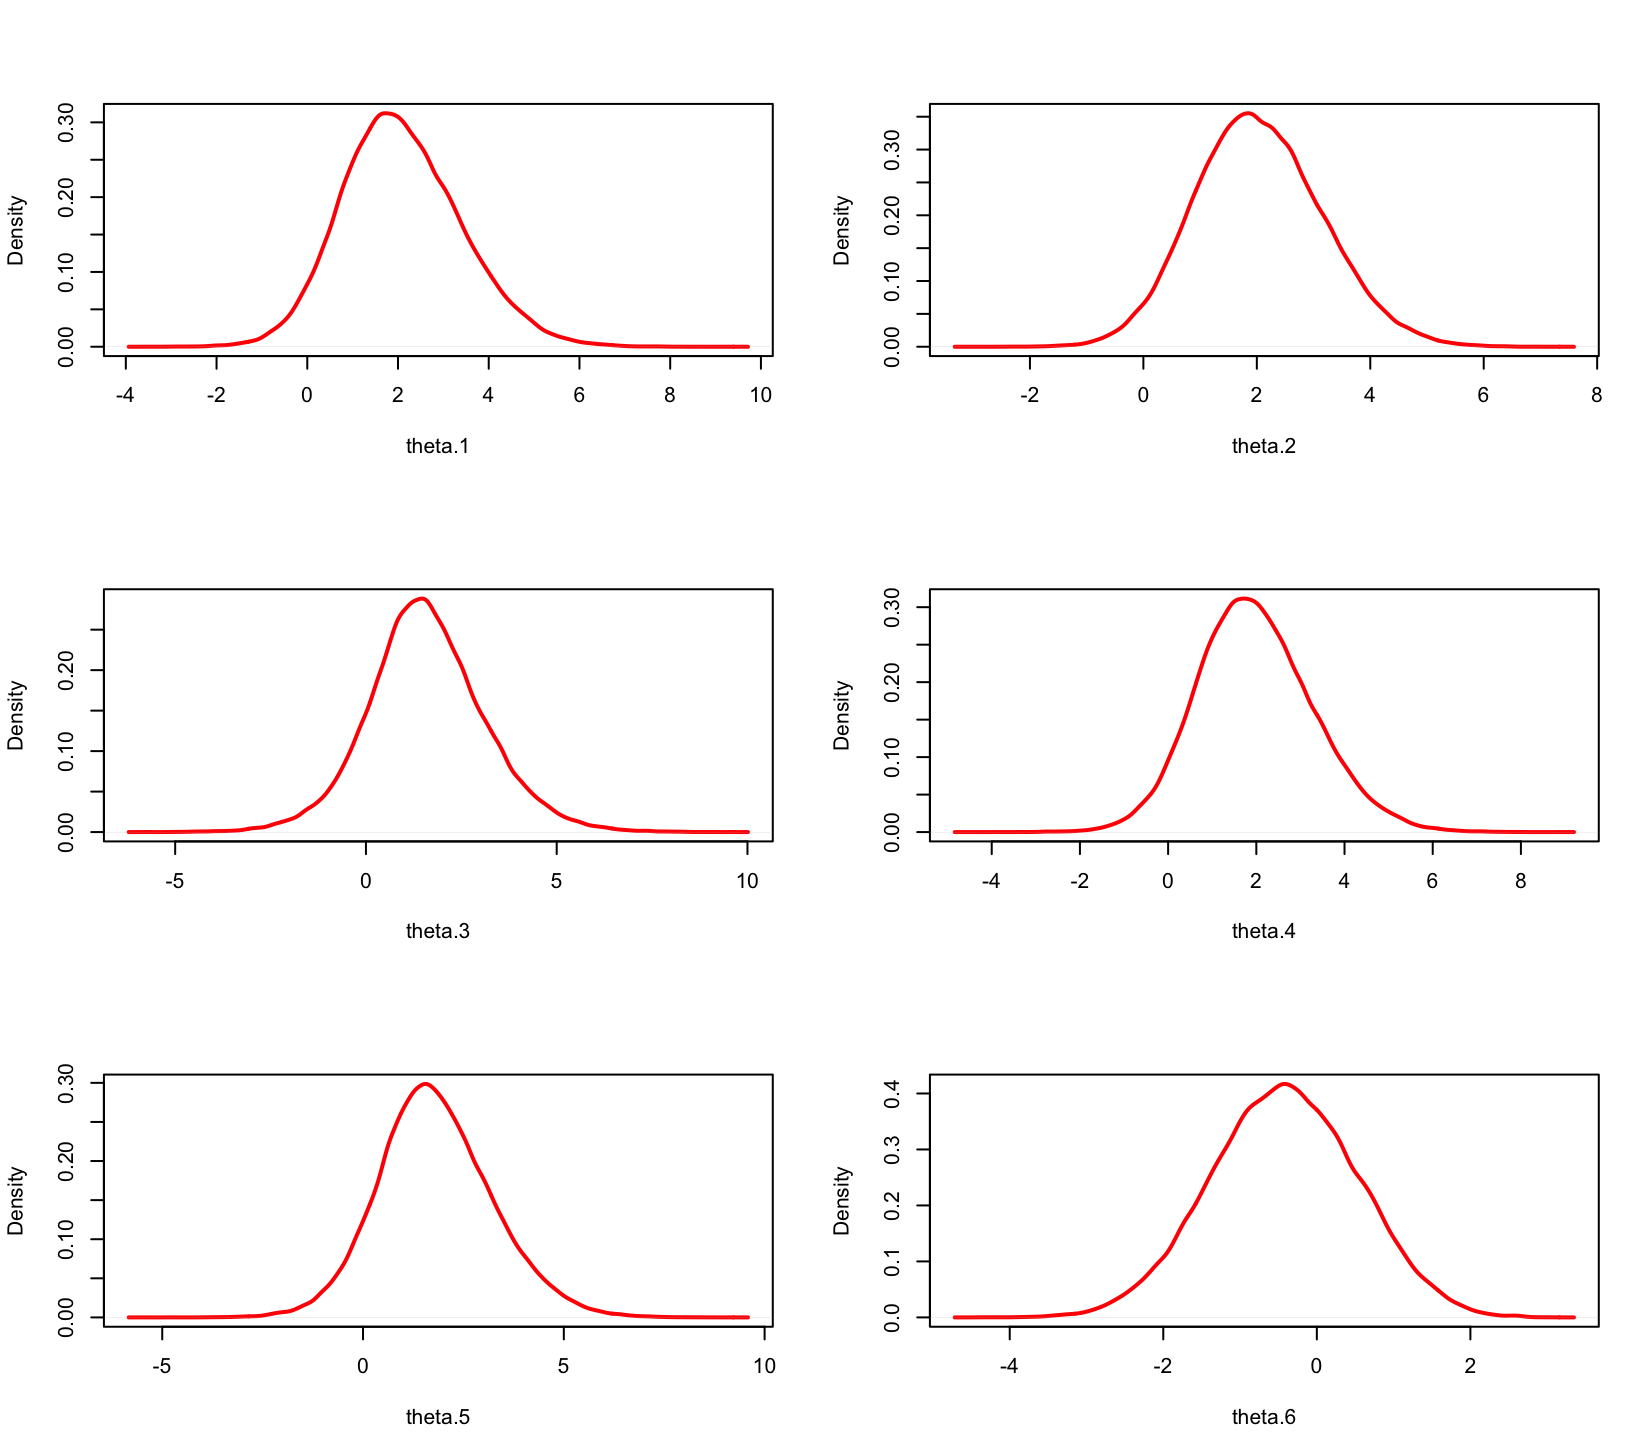
\includegraphics[scale = .3]{2Bg4.png}\]
\tcr{$\bm{END ======= 2B - g(i)(ii)(iii)======================}$}
\vspace*{1in}

\tcr{$\bm START ====== 2B - h(i)(ii) =========================$}
\begin{lstlisting}
#Used code provided
#CODE OUTPUT
Compiling model graph
   Resolving undeclared variables
   Allocating nodes
Graph information:
   Observed stochastic nodes: 6
   Unobserved stochastic nodes: 8
   Total graph size: 30

Initializing model

  |++++++++++++++++++++++++++++++++++++++++++++++++++| 100%
  |**************************************************| 100%
Mean deviance:  21.63 
penalty 4.066 
Penalized deviance: 25.7 
Compiling model graph
   Resolving undeclared variables
   Allocating nodes
Graph information:
   Observed stochastic nodes: 6
   Unobserved stochastic nodes: 1
   Total graph size: 18

Initializing model

  |++++++++++++++++++++++++++++++++++++++++++++++++++| 100%
  |**************************************************| 100%
[1] 0.2332276
[1] 0.001159899
[1] 0.95403
  |**************************************************| 100%
Mean deviance:  27.07 
penalty 1 
Penalized deviance: 28.07
\end{lstlisting}

\vspace*{1in}
\[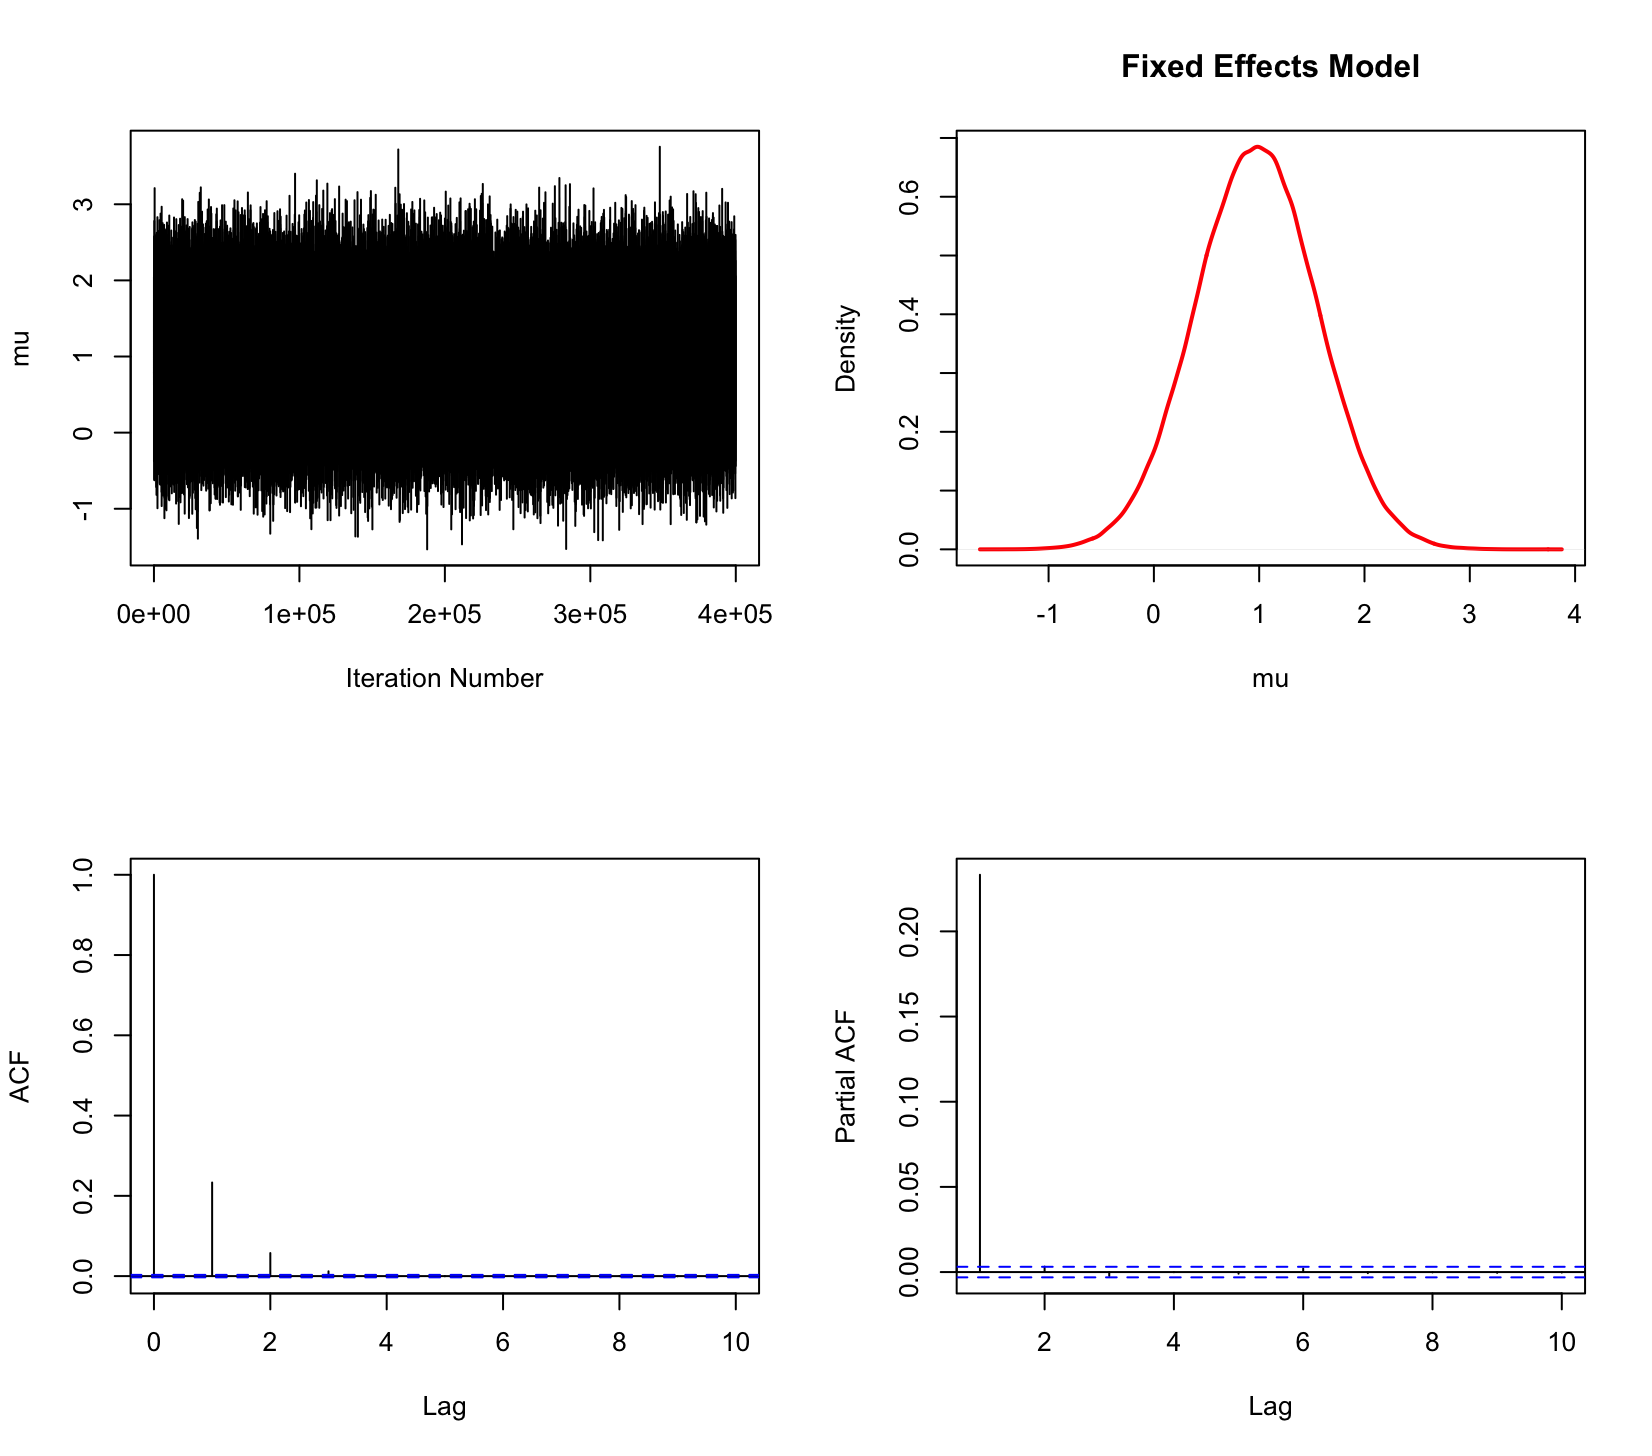
\includegraphics[scale = .3]{2Bh.png}\]

\tcr{$\bm END ====== 2B - h(i)(ii) =========================$}

\end{document}
